% NUS-style FYP report draft generated from local project materials on 2026-04-05.
% Main file only; compile with a standard LaTeX installation, e.g.:
% pdflatex nus_fyp_report_english_20260405.tex
% bibtex nus_fyp_report_english_20260405
% pdflatex nus_fyp_report_english_20260405.tex
% pdflatex nus_fyp_report_english_20260405.tex

\documentclass[12pt,a4paper]{report}

\usepackage[a4paper,margin=1in]{geometry}
\usepackage[T1]{fontenc}
\usepackage[utf8]{inputenc}
\usepackage{lmodern}
\usepackage{setspace}
\usepackage{graphicx}
\usepackage{booktabs}
\usepackage{longtable}
\usepackage{array}
\usepackage{multirow}
\usepackage{float}
\usepackage{url}
\usepackage{xurl}
\usepackage[hidelinks]{hyperref}
\usepackage[round,authoryear]{natbib}
\usepackage{enumitem}
\usepackage{caption}
\usepackage{pdflscape}

\onehalfspacing
\setcounter{secnumdepth}{3}
\setcounter{tocdepth}{2}

\title{Evaluation and Deployment of Open-Source Indoor Navigation Algorithms with Low-Cost 3D LiDAR on Mobile Platforms}
\author{NIUMU\\A0294372X}
\date{Academic Year [To be filled]}

\begin{document}

\begin{titlepage}
    \centering
    {\LARGE\bfseries Evaluation and Deployment of Open-Source Indoor Navigation Algorithms with Low-Cost 3D LiDAR on Mobile Platforms\par}
    \vspace{1.5cm}
    {\large By\par}
    \vspace{0.3cm}
    {\Large NIUMU\par}
    \vspace{0.2cm}
    {\large A0294372X\par}
    \vspace{1.2cm}
    {\large National University of Singapore\par}
    \vspace{0.8cm}
    {\large 2025/2026\par}
    \vfill
    \begin{flushleft}
    Project No.: ME5400 ROBOTICS PROJECT\\
    Supervisor: Chew Chee Meng
    \end{flushleft}
\end{titlepage}

\pagenumbering{roman}

\chapter*{Abstract}
\addcontentsline{toc}{chapter}{Abstract}
This project investigates the evaluation and deployment of open-source indoor navigation algorithms using a low-cost 3D LiDAR sensor on mobile robotic platforms. In the implemented system, a Livox MID360 LiDAR and IMU are fused with robot odometry in a unified ROS-based navigation benchmark built on \texttt{move\_base}, DWA local planning, and local/global costmaps. Four open-source LiDAR-inertial SLAM algorithms, namely LIO-SAM, FAST-LIO, Point-LIO, and FASTER-LIO, are integrated into a common navigation workflow so that they can be compared under the same robot, map, planner, and waypoint task. The broader project brief targets affordable mobile platforms including both differential-drive and tricycle-like geometries; the present implementation and experimental validation are carried out on a TurtleBot3 differential-drive platform, while the deployment workflow is designed to remain transferable to other low-cost platforms. The project makes two main contributions. First, it provides an engineering framework for standardised dataset recording, map generation, algorithm switching, rosbag-based static evaluation, and waypoint-based online navigation evaluation. Second, it studies how differences in odometry output, point-cloud representation, frame conventions, and scan generation affect downstream navigation behaviour under identical planning parameters. Static experiments on a common rosbag show that all four algorithms can localise successfully, but with different trade-offs in accuracy and computational cost. Repeated online laboratory experiments with static obstacles further show that the same planner can produce markedly different task times, safety margins, and resource profiles depending on which SLAM backend supplies odometry and obstacle observations. The final outcome is a documented, reproducible workflow for rapid deployment and system-level comparison of open-source indoor navigation pipelines on affordable mobile robot platforms.

\textbf{Subject Descriptors:} I.2.9 Robotics; C.4 Performance of Systems; I.4.8 Scene Analysis; I.5.4 Applications\\
\textbf{Keywords:} LiDAR-inertial odometry, mobile robot navigation, Livox MID360, local costmap, ROS\\
\textbf{Implementation Software and Hardware:} Ubuntu 20.04/18.04, ROS Noetic, TurtleBot3, Raspberry Pi 3, Livox MID360, LIO-SAM, FAST-LIO, Point-LIO, FASTER-LIO, \texttt{move\_base}, DWAPlannerROS, Evo

\chapter*{Acknowledgements}
\addcontentsline{toc}{chapter}{Acknowledgements}
This report summarises the implementation, debugging, and evaluation work completed on a real mobile robot platform during the Final Year Project. The author would like to express sincere gratitude to the National University of Singapore for providing the academic environment and resources that made this project possible. The author is especially grateful to the project supervisor, Chew Chee Meng, for guidance, encouragement, and valuable feedback throughout the design, integration, debugging, and evaluation stages of the work. The author would also like to acknowledge the open-source communities behind LIO-SAM, FAST-LIO, Point-LIO, FASTER-LIO, ROS navigation, and related robotics software packages, whose publicly available tools and documentation made this comparative study and reproducible engineering workflow possible.

\tableofcontents
\listoftables

\clearpage
\pagenumbering{arabic}

\chapter{Introduction}

\section{Background and Motivation}
LiDAR-inertial odometry and SLAM have become core technologies for autonomous robots that operate in environments where GNSS is unreliable and visual conditions are inconsistent. For a real mobile robot, however, high-quality odometry alone is not sufficient. A complete autonomous navigation pipeline also requires consistent coordinate frames, map generation, obstacle perception, local costmap updates, motion planning, safe velocity control, and repeatable evaluation procedures.

The Livox MID360 is attractive for such a study because it combines a compact 3D LiDAR with an IMU and is practical for deployment on a small mobile robot. At the same time, the sensor and platform combination also exposes integration difficulties that are highly relevant for robotics engineering: non-repetitive scanning patterns, frame alignment issues, topic mismatches across SLAM packages, and local obstacle updates that may fail even when SLAM itself appears to work.

This project therefore focuses not only on running a single SLAM algorithm, but on building a fair, reusable system-level benchmark in which multiple LiDAR-inertial algorithms can be compared under the same robot, same map, same planning parameters, and same waypoint task.

\section{Problem Statement}
The four candidate algorithms, LIO-SAM, FAST-LIO, Point-LIO, and FASTER-LIO, differ in their odometry topics, point-cloud outputs, frame conventions, and computational characteristics. If they are connected to navigation naively, the comparison becomes unfair: one algorithm may publish a body-frame cloud, another a map-frame cloud; one may expose a dense local cloud, another only a sparse registered map cloud; one may provide a stable odometry topic, while another exposes a higher-frequency but less suitable intermediate estimate. As a result, downstream navigation performance may differ for reasons unrelated to the underlying SLAM quality alone.

The central problem addressed by this project is therefore: \emph{How can open-source LiDAR-inertial navigation algorithms be deployed reproducibly on an affordable mobile robot equipped with a low-cost 3D LiDAR, and how can they be compared fairly at both the trajectory level and the task-execution level under shared indoor navigation tasks?}

\section{Objectives}
The project objectives are:
\begin{enumerate}[leftmargin=2em]
    \item To build a unified deployment and navigation interface for four open-source LiDAR-inertial algorithms using a common ROS navigation stack.
    \item To standardise sensor recording, map generation, and multi-algorithm startup for repeatable experiments on a low-cost mobile robot platform.
    \item To construct both static rosbag evaluation and online waypoint navigation evaluation pipelines across multiple indoor scenarios.
    \item To study how LiDAR, IMU, and odometry fusion outputs affect practical deployment properties such as map building, localisation, obstacle avoidance, and user-facing reproducibility.
    \item To identify and solve engineering issues that prevent fair comparison, especially those involving TF trees, scan generation, local costmap updates, and unstable process shutdown.
    \item To produce a report-ready archive of data, scripts, maps, TF trees, videos, and evaluation summaries.
\end{enumerate}


\section{Research Questions}
To keep the study focused and reportable, the project was guided by four research questions.
\begin{enumerate}[leftmargin=2em]
    \item How much effort is required to turn four open-source LiDAR-inertial SLAM packages into a reproducible indoor navigation benchmark rather than a collection of individually working demos?
    \item When all algorithms are connected to the same ROS navigation stack, which parts of the behaviour difference come from the planner configuration and which parts come from upstream odometry and cloud characteristics?
    \item What engineering choices are necessary to make local obstacle perception work reliably when a 3D LiDAR is converted into a 2D scan for classical indoor navigation?
    \item Can a low-cost mobile robot platform support a workflow that is sufficiently standardised to compare algorithms fairly across multiple indoor scenarios such as a laboratory, an outdoor open area, and a long corridor?
\end{enumerate}

These questions are important because open-source robotics projects often demonstrate isolated algorithm performance but provide only limited guidance on reproducible deployment. In practice, students and engineers frequently spend more time on frame alignment, rosbag hygiene, process management, and costmap debugging than on the algorithm paper itself. The present report therefore treats deployment knowledge as a research contribution in its own right.

\section{Contributions}
The main contributions of the project are as follows:
\begin{enumerate}[leftmargin=2em]
    \item A unified SLAM-to-navigation integration framework based on the common topics \path{/slam/odom} and \path{/slam/cloud_registered}.
    \item A practical toolchain for remote deployment, rosbag recording, map export, static trajectory evaluation, and online waypoint evaluation.
    \item A documented debugging methodology for scan/costmap failures, TF inconsistencies, rosbag replay jitter, and process cleanup issues.
    \item A benchmark dataset archive under the local \texttt{FYP} directory, including bags, generated maps, TF tree snapshots, obstacle-avoidance videos, and evaluation outputs.
    \item A comparative analysis showing how upstream SLAM outputs affect downstream navigation behaviour even when the planner parameters are held constant.
\end{enumerate}

\chapter{Related Work}

\section{International Research on LiDAR SLAM and Navigation}
Classical LiDAR odometry and mapping was strongly shaped by LOAM, which separated the front-end odometry and back-end mapping processes to achieve real-time performance with relatively low drift \citep{zhang2017loam}. LOAM established the practical importance of using geometric features extracted from point clouds and remains a conceptual reference point for many later LiDAR-based systems.

LeGO-LOAM extended this family in a direction that is especially relevant for deployment on small robots: it simplified the pipeline around ground segmentation and lightweight terrain-aware processing, making it attractive for embedded or compute-constrained platforms \citep{shan2018legoloam}. This is important in the context of the present project because the broader goal is not merely to show that a SLAM algorithm works once, but to understand which methods remain practical when carried onto a modest mobile base with limited onboard resources and non-ideal wiring, power, and communication conditions.

For robot navigation, the Dynamic Window Approach (DWA) remains one of the most influential local planning methods. It searches directly in velocity space while respecting robot dynamics and obstacle constraints, and forms the conceptual basis of the \texttt{DWAPlannerROS} implementation used in this project \citep{fox1997dwa}.

Among more recent LiDAR-inertial methods, LIO-SAM introduced a factor-graph formulation that tightly couples LiDAR odometry, IMU preintegration, and mapping, while allowing loop closure and multiple measurement sources to be fused consistently \citep{shan2020liosam}. LIO-SAM is especially influential because it balances real-time performance with graph-based smoothing and has become widely adopted in ROS-based research prototypes.

FAST-LIO2 represents a different design philosophy. Instead of maintaining a feature-heavy mapping backend, it pushes toward a highly efficient iterated Kalman filter formulation with raw-point registration and an incremental kd-tree structure \citep{xu2022fastlio2}. Point-LIO and FASTER-LIO continue this trend in different directions: Point-LIO emphasises point-wise high-bandwidth state updates for aggressive motion, while FASTER-LIO focuses on sparse incremental voxels and reduced runtime burden \citep{he2023pointlio,bai2022fasterlio}. Together, these methods highlight a broader shift in LiDAR-inertial research from purely geometric accuracy toward latency, resource efficiency, and robustness under real platform motion.

Another nearby branch is LiDAR-inertial-visual fusion. Systems such as FAST-LIVO, FAST-LIVO2, R$^3$LIVE, and R$^3$LIVE++ expand beyond LiDAR and IMU by using camera observations for texture, radiance, or additional geometric constraints \citep{zheng2022fastlivo,zheng2024fastlivo2,lin2022r3live,lin2024r3livepp}. These systems are highly relevant from a research perspective because they show how richer sensing can improve robustness and map quality. At the same time, they also make the deployment burden heavier by introducing camera calibration, exposure management, and visual tracking assumptions. This project therefore treated them as important reference points during scoping, but not as the final implementation target for the unified benchmark, because the stated project aim emphasises robust deployment on low-cost platforms rather than the most sensor-rich pipeline available.

More broadly, recent reviews show that SLAM research has moved increasingly toward domain-aware and deployment-oriented systems, where practical concerns such as sensor configuration, computational load, and robustness in changing environments are as important as raw localisation accuracy \citep{yarovoi2024review}.

This deployment-oriented reading is also consistent with broader mobile-robot positioning surveys. Reviews of indoor positioning methods show that algorithm choice cannot be separated from constraints such as infrastructure cost, calibration effort, robustness to layout changes, and the amount of environmental modification required \citep{huang2023indoorpositioningreview}. For the present project, this observation is central: the report is not only about which open-source package obtains the lowest trajectory error, but also about which package can be connected to a shared navigation stack with the smallest amount of special-case engineering.

\section{Broader Algorithm Landscape Considered During Scoping}
Before narrowing the implementation to four core algorithms, a broader survey of open-source navigation and SLAM candidates was carried out. Early project notes and weekly progress materials show that the investigation initially covered not only LOAM, LIO-SAM, FAST-LIO, Point-LIO, and FASTER-LIO, but also LeGO-LOAM, FAST-LIVO, FAST-LIVO2, R3LIVE, and R$^3$LIVE++ as representative examples of different sensing and fusion philosophies.

This broader survey was useful for two reasons. First, it clarified that available open-source systems differ not only in estimation backend but also in sensor assumptions. Some are LiDAR-only, some are LiDAR-inertial, and others rely on tightly integrated visual measurements. Second, it made clear that a project centred on affordable indoor deployment should prioritise algorithms that are realistic to calibrate, reproduce, and maintain on a small mobile robot. As a result, the final implementation deliberately focused on LiDAR-inertial pipelines that could be connected to the same robot and navigation stack without introducing an additional camera calibration and visual-tracking burden.

The survey also helped refine the evaluation criteria. In the early phase, speed and accuracy were the most obvious criteria. Over time, however, deployment-oriented factors became equally important: whether the method could work with the available IMU data format, whether the required point-cloud message structure could be generated from the chosen sensor, whether the algorithm depended on sensor-specific metadata such as ring indices, whether map building was streamlined enough for student use, and whether the algorithm could be integrated into an operator-friendly launch workflow. This shift from purely algorithmic novelty to deployment practicality strongly influenced the final project scope.

\begin{figure}[H]
\centering
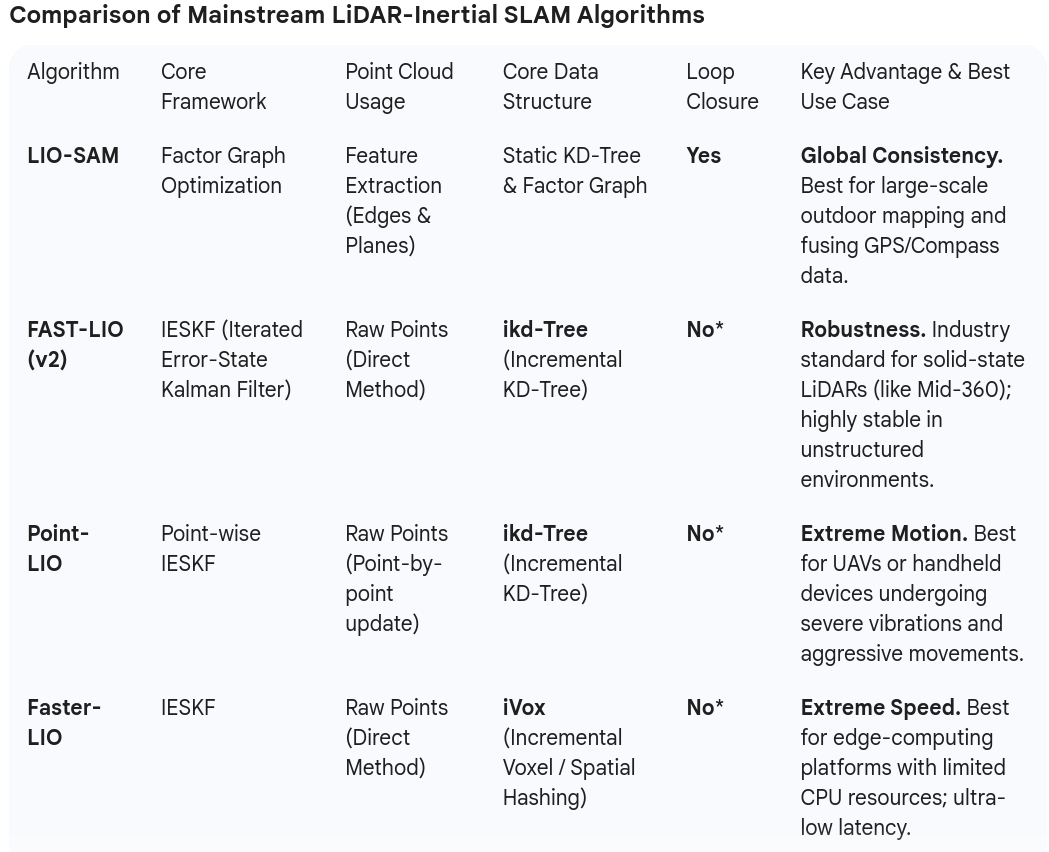
\includegraphics[width=0.9\textwidth]{report_assets/ppt_media_all/image48.png}
\caption{Algorithm comparison slide consolidated during the project scoping stage. The weekly project presentation materials were reviewed in full and used here as evidence of the broader algorithm landscape considered before the benchmark was narrowed to four LiDAR-inertial methods.}
\label{fig:ppt-algorithm-landscape}
\end{figure}

\section{Regional and Domestic Research Status}
Research groups in Hong Kong and mainland China have made especially strong contributions to tightly coupled LiDAR-inertial odometry in recent years. FAST-LIO2, developed by the University of Hong Kong, shifted away from hand-crafted feature extraction and instead registered raw points directly to the map using an iterated Kalman filter and incremental kd-tree map management, achieving strong efficiency and adaptability across sensor types \citep{xu2022fastlio2}.

Point-LIO further pushed the emphasis on update frequency and aggressive motion handling by introducing point-by-point state updates and a stochastic-process-based formulation for handling high-bandwidth motion and IMU saturation \citep{he2023pointlio}. In parallel, FASTER-LIO pursued computational efficiency through parallel sparse incremental voxels and lightweight tracking, aiming to retain accuracy while reducing runtime burden \citep{bai2022fasterlio}.

These works demonstrate that recent regional research is not only about improving localisation accuracy, but also about improving update rate, robustness to aggressive motion, and suitability for real robotic platforms with limited computation. This trend is directly relevant to the present project, which evaluates not just SLAM trajectories, but the effect of each algorithm on a full robot navigation stack.

\section{Gap Addressed by This Project}
Most algorithm papers evaluate localisation accuracy on public datasets and focus primarily on odometry or mapping metrics. By contrast, this project studies the system-level gap between SLAM outputs and real navigation behaviour. In particular, it asks how different choices of odometry topic, point-cloud topic, and frame convention influence scan generation, local costmap updates, obstacle clearance, completion time, and command smoothness. This project therefore complements algorithm-level evaluation with a downstream navigation benchmark under a unified experimental platform.

A second gap concerns deployment on affordable robotic hardware. In many academic publications, the boundary between the algorithm and the surrounding engineering stack is intentionally simplified so that the core estimation method can be highlighted. In a student project built on real hardware, however, the engineering stack is inseparable from the final outcome. Sensor wiring, topic naming, remote deployment, data recording, map generation, and experiment reset procedures all affect whether a navigation experiment is repeatable. The report therefore deliberately documents these engineering layers rather than treating them as peripheral implementation detail.

A third gap concerns scenario diversity. A single static indoor map is useful for baseline comparison, but it cannot reveal all relevant weaknesses. An algorithm that performs well in a laboratory may behave differently in an open outdoor space or a narrow corridor because the geometric structure, obstacle distribution, and local costmap demands are different. For this reason, the project report is structured around three scenarios so that the final comparison can discuss not only which algorithm is more accurate in isolation, but also which algorithm is more suitable for a given deployment context.

\chapter{System Overview}

\section{Hardware Platform}
The physical platform used in this project consists of three main hardware components.

\subsection{TurtleBot3 Mobile Base}
The robot base used for implementation and evaluation is a TurtleBot3 differential-drive platform. TurtleBot3 provides an open ROS-compatible mobile base, compact footprint, and convenient integration for navigation and teleoperation experiments. It is well suited for indoor benchmarking because the chassis, wheelbase, and control stack are widely used and easy to reproduce. The broader project brief also considers mobile robots with tricycle steering geometry and one steerable driving wheel; although such a platform was not the primary experimental base in the present archive, the deployment methodology developed in this project was intentionally organised around reusable ROS interfaces so that the workflow can be transferred to other affordable mobile platforms.

\subsection{Raspberry Pi 3 Onboard Computer}
A Raspberry Pi 3 is used as the onboard computer on the robot side. Its role in the project is to support base-related communication and platform-side ROS integration, while more computationally expensive SLAM, visualisation, and analysis tasks are executed on an external workstation through a multi-machine ROS configuration. This division of labour reflects a realistic deployment scenario in which the robot carries lightweight onboard computing while high-load LiDAR-inertial processing may still depend on a stronger host machine.

\subsection{Livox MID360 LiDAR and IMU}
The main perception sensor is the Livox MID360, which provides 3D LiDAR measurements together with IMU data. In this project, the MID360 serves as the common sensing source for all four SLAM algorithms. Its compact form factor makes it practical for the TurtleBot3 platform, while its LiDAR-plus-IMU design makes it suitable for tightly coupled LiDAR-inertial odometry.

\begin{figure}[H]
\centering
\begin{minipage}[t]{0.32\textwidth}
\centering
\includegraphics[width=\linewidth]{report_assets/ppt_media_all/image21.jpeg}
\end{minipage}\hfill
\begin{minipage}[t]{0.32\textwidth}
\centering
\includegraphics[width=\linewidth]{report_assets/ppt_media_all/image22.jpeg}
\end{minipage}\hfill
\begin{minipage}[t]{0.32\textwidth}
\centering
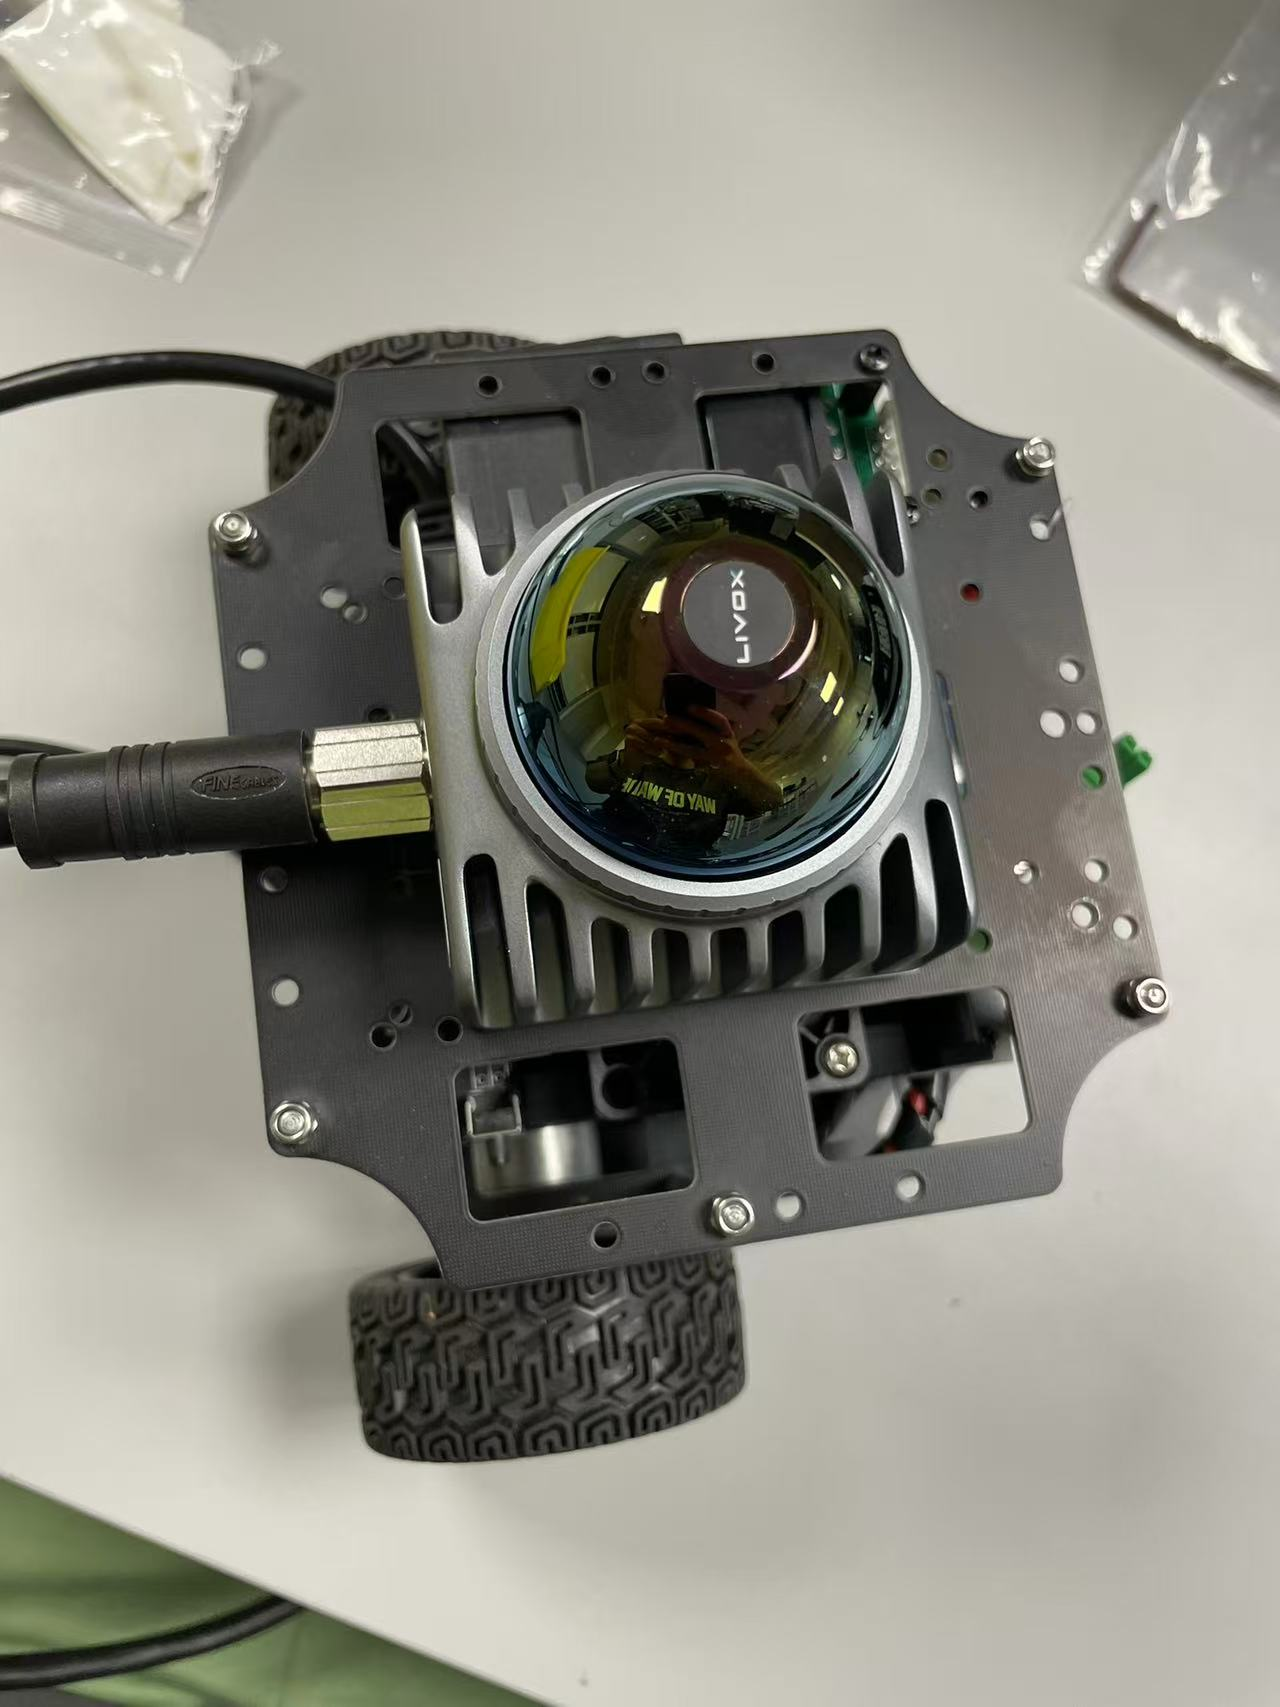
\includegraphics[width=\linewidth]{report_assets/ppt_media_all/image41.png}
\end{minipage}
\caption{Hardware platform materials reviewed from the weekly project archive: the TurtleBot3-based experimental setup, onboard wiring and mounting, and the Livox MID360 installation. These images are useful because they document the real deployment context rather than a purely simulated configuration.}
\label{fig:hardware-platform}
\end{figure}

\section{Early Hardware Integration Challenges}
The hardware bring-up phase exposed several practical problems that later shaped the system design. Weekly project materials recorded multiple issues on the TurtleBot3--Raspberry Pi 3 platform: insufficient onboard memory during compilation, the need to enlarge swap space to complete catkin builds, potentially unsafe power and connector arrangements around the LiDAR and battery wiring, and the importance of reliable Ethernet/RJ45 connectivity for remote operation. These issues are not cosmetic details. They directly affect whether a low-cost platform can be deployed repeatedly and safely in a lab environment.

The Raspberry Pi 3 in particular imposed constraints on compilation and runtime management. Early experiments showed that parallel compilation could exhaust available memory and lead to the platform becoming unresponsive or shutting down. This motivated more conservative build settings and a swap-space workaround during setup. Similarly, remote SSH-based keyboard control became part of the practical workflow because local interaction with the onboard computer was inconvenient once the platform was assembled with sensor payload and cabling.

The Livox MID360 integration also involved non-trivial sensor adaptation work. Earlier progress records indicate that the project had to consider issues such as IMU dimensionality assumptions, point-cloud message compatibility with ROS processing pipelines, and missing ring information needed by some LiDAR algorithms. These adaptation issues reinforced the broader lesson that low-cost sensor deployment is not just a matter of selecting an algorithm from the literature; it requires substantial middleware and data-format engineering before a fair navigation comparison is even possible.

\begin{figure}[H]
\centering
\begin{minipage}[t]{0.48\textwidth}
\centering
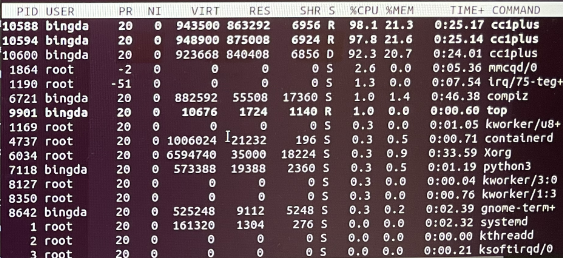
\includegraphics[width=\linewidth]{report_assets/ppt_media_all/image25.png}
\end{minipage}\hfill
\begin{minipage}[t]{0.48\textwidth}
\centering
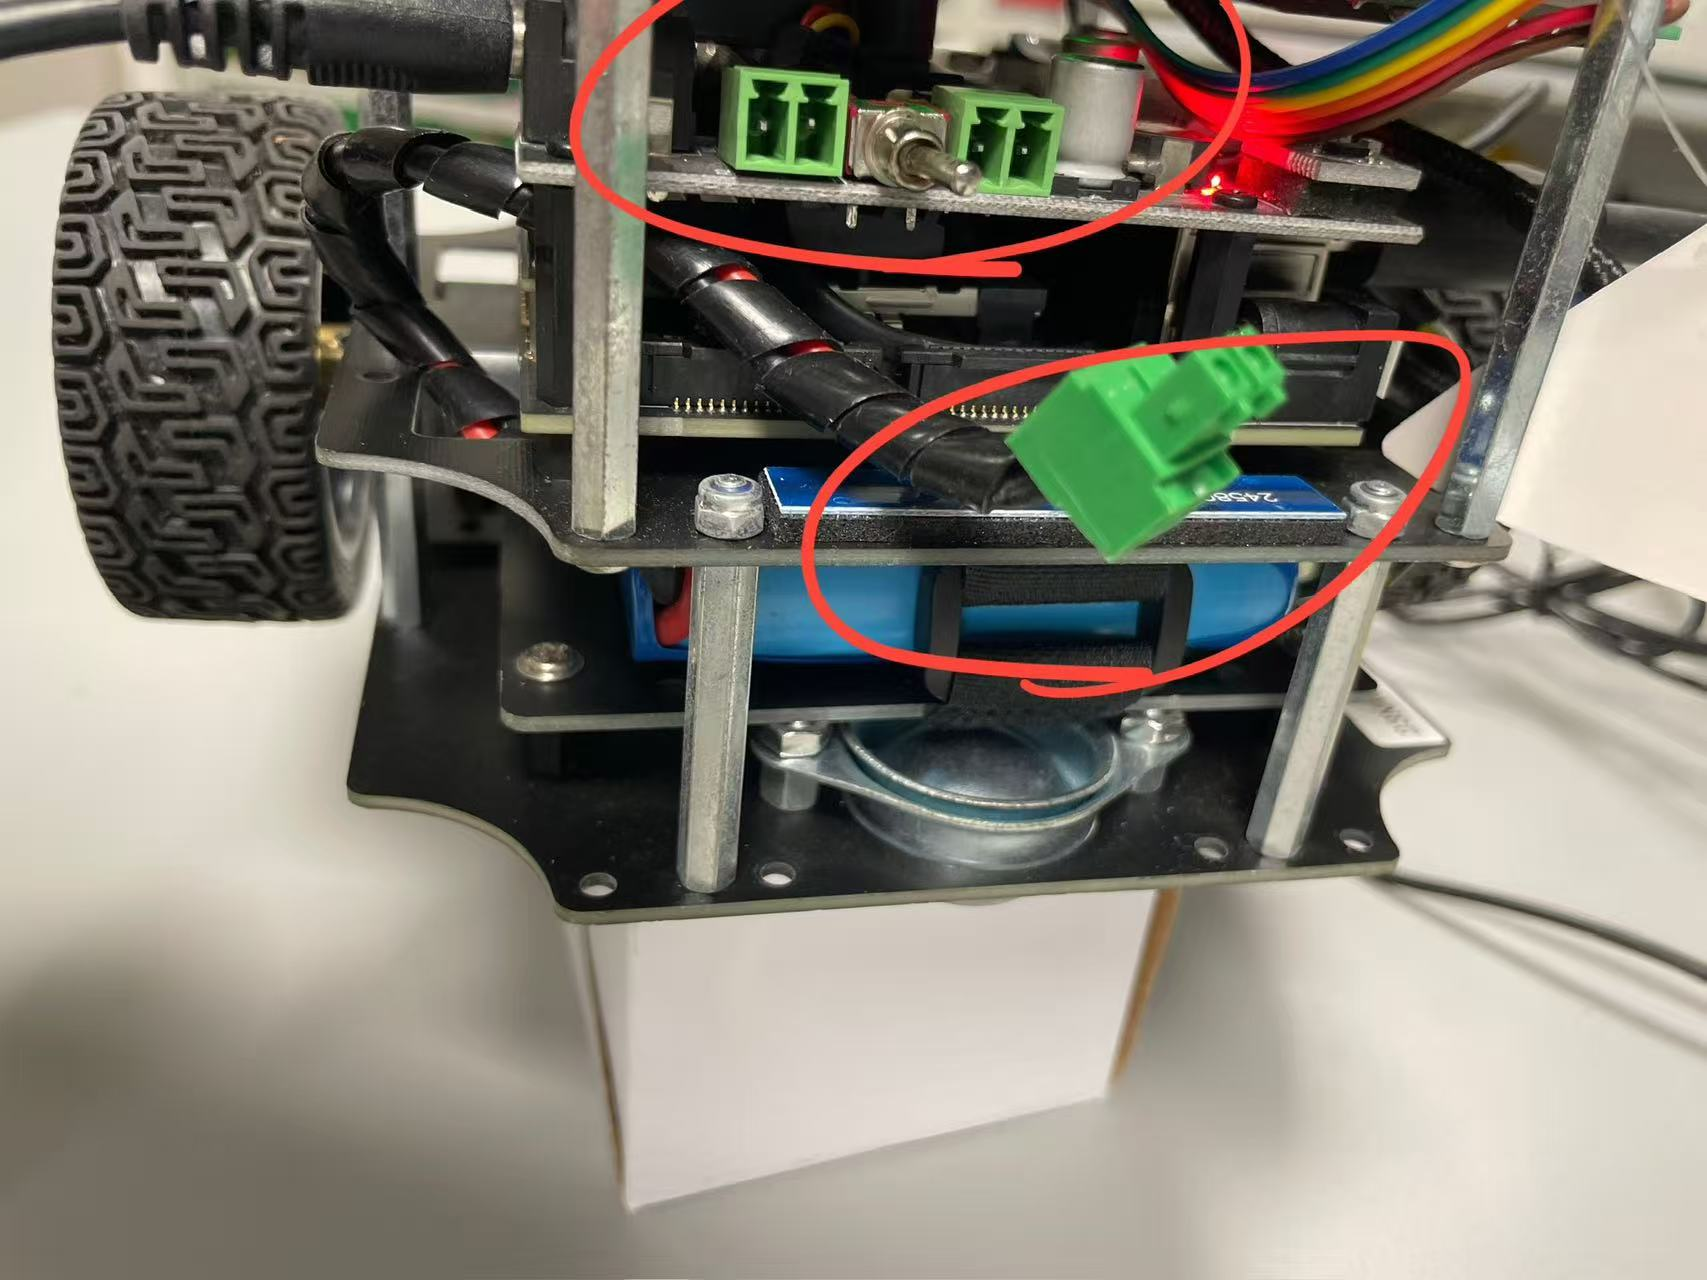
\includegraphics[width=\linewidth]{report_assets/ppt_media_all/image37.png}
\end{minipage}
\caption{Examples of early hardware integration constraints documented in the weekly project presentation: Raspberry Pi resource limitations during compilation and a power-cable arrangement that had to be treated as a safety issue during bring-up.}
\label{fig:hardware-challenges}
\end{figure}

\section{Software Stack}
The software stack is based on ROS Noetic and a standard navigation architecture consisting of a static occupancy-grid map, \texttt{pointcloud\_to\_laserscan} for obstacle observation generation, \texttt{move\_base} with global and local costmaps, and \texttt{DWAPlannerROS} as the local planner. The robot and workstation were operated in a multi-machine ROS configuration during real-world experiments, with the robot hosting the sensor and base drivers and the workstation used for visualisation, data analysis, and batch evaluation. Although the wider project description mentions EKF/UKF-based fusion as representative solution families, the implemented comparison in this report focuses on four open-source LiDAR-inertial SLAM pipelines that were actually integrated and evaluated in the local project archive.


\section{Design Constraints and Practical Assumptions}
Several practical constraints shaped the system design. First, the platform is cost-sensitive: the robot base, onboard computation, and sensor suite should remain affordable and easy to reproduce. Second, the robot uses a classical ROS navigation stack rather than a custom planner, because the goal of the project is not to invent a new local planner but to compare how different open-source odometry pipelines behave under a common navigation backend. Third, the benchmark must be easy to reset between trials, which means that process cleanup, map reuse, and standardised launch sequences are not optional conveniences but core parts of the experiment design.

A further assumption is that the evaluation should remain meaningful even if not every internal component is made identical across all algorithms. In other words, the project does not force each algorithm to publish exactly the same native outputs. Instead, it standardises the interface that navigation consumes and then documents the algorithm-specific bridging decisions. This preserves engineering realism while keeping the comparison interpretable.

\section{Unified Navigation Interface}
A major engineering contribution of the project is the introduction of a common interface layer so that all four SLAM algorithms can be swapped without changing the navigation stack itself. The common interface consists of two topics:
\begin{enumerate}[leftmargin=2em]
    \item \texttt{/slam/odom} for odometry input to navigation, and
    \item \texttt{/slam/cloud\_registered} for point-cloud input used to generate \texttt{/scan}.
\end{enumerate}

The unification is performed through lightweight relay nodes and algorithm-specific startup logic. The current archived integration strategy is summarised in Table~\ref{tab:unified-interface}.

\begin{table}[H]
\centering
\caption{Unified interface used to connect four SLAM algorithms to the same navigation stack.}
\label{tab:unified-interface}
\setlength{\tabcolsep}{4pt}
\renewcommand{\arraystretch}{1.05}
\resizebox{\linewidth}{!}{%
\begin{tabular}{llll}
\toprule
Algorithm & Native odometry used & Native cloud used for navigation & Scan frame \\
\midrule
LIO-SAM & \texttt{/odometry/imu} & \texttt{/lio\_sam/mapping/cloud\_registered\_raw} & \texttt{base\_link} \\
FAST-LIO & \texttt{/Odometry} & \texttt{/cloud\_registered} & \texttt{base\_link} \\
Point-LIO & \texttt{/aft\_mapped\_to\_init} & \texttt{/cloud\_registered\_body} & \texttt{base\_link} \\
FASTER-LIO & \texttt{/Odometry} & \texttt{/cloud\_registered\_body} & \texttt{base\_link} \\
\bottomrule
\end{tabular}
}
\end{table}

\section{TF Tree Harmonisation}
The four algorithms do not expose identical TF trees or output topics. Therefore, the project standardised the downstream navigation assumptions around a common robot body frame, \texttt{base\_link}, and a common global frame pair \texttt{map \textrightarrow odom \textrightarrow base\_link}.

The archived baseline TF tree snapshots are stored under the local project archive and include one PDF for each algorithm. Local configuration inspection shows that FAST-LIO and FASTER-LIO explicitly define \path{map_frame = map} and \path{body_frame = base_link}, while Point-LIO can publish a body-frame cloud when \path{scan_bodyframe_pub_en} is enabled. LIO-SAM currently uses \path{lidarFrame = base_link}, \path{baselinkFrame = base_link}, \path{odometryFrame = odom}, and \path{mapFrame = map}. The project did explore a more explicit \path{livox_frame} alignment for LIO-SAM, but that change was later rolled back to preserve a stable baseline for comparison.

The practical lesson is that fair comparison does not require all internal algorithm frames to be identical. It does, however, require a stable downstream contract: navigation must always know which odometry topic and which cloud topic to trust, and those topics must be consistent with the scan frame used by \texttt{pointcloud\_to\_laserscan} and the obstacle layer.

\section{Obstacle Observation Chain}
Obstacle handling in the navigation stack follows the chain below:
\begin{enumerate}[leftmargin=2em]
    \item the selected SLAM point cloud is bridged to \texttt{/slam/cloud\_registered},
    \item \texttt{pointcloud\_to\_laserscan} converts it into \texttt{/scan},
    \item the local obstacle layer consumes \texttt{/scan}, and
    \item the local costmap is updated for DWA-based avoidance.
\end{enumerate}

Much of the debugging effort in this project focused on this chain. In several cases, the SLAM algorithm itself was working, but the local costmap failed because the cloud was too sparse, in the wrong frame, or not appropriate for real-time 2D obstacle extraction.

\chapter{Implementation and Engineering Toolchain}

\section{Recording and Dataset Management}
A standardised data recording launch file was created to make real-world experiments repeatable. The recording pipeline performs three tasks at once: it smooths raw teleoperation commands before they reach the base controller, publishes required static transforms and a unified odometry topic, and records LiDAR, IMU, odometry, TF, and TF-static topics into rosbag files. This standardisation was essential for later ATE/RPE computation, because early bags did not contain a suitable ground-truth topic.

\section{Unified Startup Scripts}
A unified startup script was developed so that each SLAM algorithm can be launched together with navigation using the same external interface. This script also performs cleanup of residual ROS nodes and relay processes so that repeated experiments do not inherit stale processes from previous runs. This was a necessary engineering step because process residue was repeatedly found to cause false failures, duplicated TFs, and costmap warnings.

\section{Remote Deployment and Multi-Machine Operation}
A substantial part of the project involved making the workflow deployable rather than only executable on a single development machine. The robot and the workstation operate in a multi-machine ROS configuration, with the robot handling base-side communication and sensor-side processes while the external workstation handles heavier SLAM, visualisation, and batch evaluation tasks. This division is especially important for a Raspberry Pi 3 based platform, where computational headroom is limited.

To make this workflow repeatable, remote deployment scripts were developed so that the same package set could be synchronised, permissioned, and built consistently on the robot side. This reduced the risk of version drift between the workstation and the robot and enabled quicker iteration when navigation scripts, launch files, or evaluation utilities were updated.

\section{Topic Normalisation and Interface Bridging}
The four algorithms differ in both naming and semantics of their outputs. Some provide a map-frame registered cloud, while others can provide a body-frame cloud that is more suitable for local obstacle extraction. Some expose high-rate odometry estimates, while others expose more stable mapping outputs. If these differences are ignored, the navigation comparison becomes difficult to interpret.

The project therefore introduced a normalisation layer based on two common downstream topics: \texttt{/slam/odom} and \texttt{/slam/cloud\_registered}. Lightweight relay nodes were used so that the navigation stack could remain unchanged when the SLAM backend was switched. This may appear simple at first sight, but much of the debugging history showed that choosing the wrong source cloud, especially a world-frame cloud in place of a body-frame cloud, had a direct impact on whether \texttt{/scan} was responsive enough for local obstacle avoidance.

\section{Motion Smoothing for Repeatable Recording}
The project also identified a gap between teleoperation convenience and dataset quality. Raw keyboard teleoperation can produce abrupt velocity steps that are acceptable for quick manual driving but undesirable for reproducible evaluation. To address this, a command smoother was inserted between the raw teleoperation source and the final base command topic. The smoother applies acceleration and deceleration limits to both linear and angular velocity, which improves driver consistency, reduces abrupt chassis motion, and leads to cleaner recorded bags.

This smoothing step became especially important because the recorded bags were later reused for offline SLAM evaluation and map generation. Better driving quality produced cleaner and more representative datasets, which in turn reduced the risk of attributing poor results to an algorithm when the underlying bag itself was unnecessarily aggressive or noisy.

\section{Experiment Automation and Cleanup}
A recurring problem during development was that ROS processes from earlier runs continued to exist in the background and interfered with later experiments. These leftovers included relay nodes, navigation processes, and launch parents that continued to publish topics or respawn children after the operator believed the run had ended. Such residue created misleading warnings, duplicated node names, and repeated local costmap errors.

To control this, the unified startup and evaluation scripts were gradually extended to include stronger cleanup logic. The result was an experiment workflow that is closer to a benchmark harness than an ad hoc launch recipe. This matters for the report because reproducibility in robotics is often undermined by process-state artefacts rather than by the algorithm alone.

\section{Static Evaluation Pipeline}
The static evaluation pipeline automates the replay of a common rosbag for each SLAM algorithm, exports trajectories to TUM format, runs APE/RPE evaluation, and records resource usage and frame timing. The result directory structure contains per-algorithm logs, estimated trajectories, evaluation text outputs, and a machine-generated summary table.

\section{Online Waypoint Evaluation Pipeline}
A separate waypoint evaluation tool publishes goals to the navigation stack and records task-level performance metrics such as success rate, total completion time, average speed, minimum scan distance, near-collision count, recovery count, command smoothness, and CPU/GPU usage. The evaluator also supports appending the robot start pose as a final goal, which makes return-to-start error measurable without manually duplicating the first waypoint.

\section{Map Generation from PCD}
The project includes a utility to convert 3D PCD maps into 2D occupancy maps without overwriting the default navigation map. This capability was used to generate new maps from saved point clouds while preserving a stable reference map for baseline experiments.

\chapter{Experimental Methodology}

\section{Project Assets Reviewed for This Report}
All currently archived FYP materials relevant to the report were reviewed. The local archive includes rosbags, exported PCD map folders, TF tree snapshots, online waypoint evaluation outputs, static rosbag evaluation outputs, waypoint definitions, obstacle-avoidance videos, and earlier project presentation materials documenting preliminary literature review and hardware bring-up. Together, these artefacts form the empirical basis of the present report.

\section{Static Rosbag Evaluation}
The static evaluation uses a common recorded rosbag and runs each SLAM algorithm separately on identical sensor input. The outputs are converted to trajectory files and compared against the recorded reference odometry. The primary metrics are ATE RMSE, RPE RMSE, mean CPU usage, mean memory usage, mean frame time, and odometry message count. This evaluation isolates localisation and computational behaviour without the confounding influence of the navigation stack.

\section{Online Waypoint Navigation Evaluation}
The online navigation evaluation is structured around three representative deployment scenarios rather than a single route. In all cases, the same robot platform, the same Livox MID360 sensor, the same ROS navigation stack, and the same DWA local planner are retained. What changes across scenarios is the map, the waypoint route, and the environmental challenge posed to obstacle perception and path execution.

\subsection{Scenario Definition}
The three scenarios used in the project are summarised in Table~\ref{tab:scenarios}.

\begin{table}[H]
\centering
\caption{Online navigation scenarios used in the project.}
\label{tab:scenarios}
\begin{tabular}{p{3cm}p{4cm}p{7cm}}
\toprule
Scenario & Environment type & Main evaluation focus \\
\midrule
Indoor laboratory map & Static indoor laboratory map generated from the lab environment & Baseline path tracking, localisation stability, repeatability, and fair same-task comparison under controlled obstacles \\
Outdoor map & Outdoor environment with larger open space and potentially weaker structural constraints & Robustness to sparser geometric constraints, odometry drift, and larger-scale route execution \\
Corridor map & Long corridor or narrow-passage environment & Tight-clearance obstacle avoidance, local costmap responsiveness, and planner behaviour under constrained geometry \\
\bottomrule
\end{tabular}
\end{table}

The currently archived route contains four manually captured goals, and the evaluator can append the start pose as a final goal, effectively creating a five-goal sequence with a return-to-start test. This route definition is reused scenario-by-scenario so that each algorithm is assessed under comparable task structure even when the map changes.

The primary online metrics are:
\begin{enumerate}[leftmargin=2em]
    \item success count and success rate,
    \item total completion time,
    \item total travelled path length,
    \item average speed,
    \item minimum scan distance to obstacles,
    \item average goal position error,
    \item average goal yaw error,
    \item recovery count,
    \item near-collision count,
    \item command smoothness, and
    \item system CPU/GPU usage.
\end{enumerate}

\section{Metric Rationale}
The selected metrics were chosen to reflect both algorithmic and user-facing behaviour. Success rate is the most direct measure of whether a navigation pipeline can complete a task at all. Total completion time and average speed reflect practical efficiency, while travelled path length reveals whether an algorithm-planner combination tends to take detours. Minimum scan distance and near-collision count capture safety and clearance behaviour, which are especially relevant in narrow indoor spaces. Recovery count provides a compact proxy for how often navigation becomes uncertain or trapped. Goal position and yaw errors reflect task accuracy, and command standard deviation provides insight into motion smoothness and whether the robot moves in a stable or jittery manner.

CPU and GPU measurements are included because deployment on low-cost hardware depends not only on accuracy but also on resource affordability. An algorithm that localises slightly better but requires substantially higher compute may be less attractive for practical deployment on a lightweight mobile robot. The project therefore treats computational demand as part of deployment quality rather than as a secondary statistic.

\section{Trial Protocol and Repeatability}
For each scenario, the intended protocol is to keep the map fixed, keep the waypoint route fixed, and keep the navigation parameters fixed while changing only the SLAM backend and its justified bridge topics. The robot should start from approximately the same pose at the beginning of each run, and environmental disturbance should be kept similar across runs whenever possible. In the laboratory scenario, this is easier to control because the environment is largely static. In the corridor and outdoor scenarios, stricter note-taking is needed to record whether obstacles, pedestrians, or route obstructions changed between trials.

The online evaluator further standardises the route by reading a waypoint file in the map frame and optionally appending the start pose as a final goal. This feature turns return-to-start consistency into a measurable quantity and makes route completion more informative than a one-way test. The evaluator also records timeline logs, per-goal summaries, and run-level summaries so that both numerical tables and debugging narratives can be reconstructed after the experiment.

\section{Scenario-Specific Hypotheses}
The three scenarios are not included merely to enlarge the experiment count; each one is expected to reveal a different failure mode or strength. In the indoor laboratory map, the main expectation is that all algorithms should be able to complete the route once integration is correct, so differences are likely to appear in smoothness, safety margin, and computational profile. In the outdoor map, the expectation is that drift sensitivity, reduced structural richness, and larger route scale will become more important. In the corridor scenario, the working hypothesis is that cloud choice and scan responsiveness will dominate the result because narrow-space avoidance relies heavily on a well-updated local costmap.

These scenario-specific hypotheses are useful because they turn the benchmark from a simple leaderboard into an explanatory framework. Rather than asking only which algorithm is best overall, the report can ask which algorithm is more suitable for a constrained corridor, which is more robust in an open environment, and which offers the most deployment-friendly balance in a baseline indoor map.

\section{Fairness Considerations}
To keep the comparison as fair as possible, the project controlled the following variables across runs: identical robot platform and sensor suite, identical planner and costmap configuration, identical map-loading procedure within each scenario, and standardised odometry/cloud topic bridging. At the same time, the report explicitly recognises that system-level comparison is inherently affected by the type of cloud and odometry each algorithm exposes. This is not a flaw in the study; it is part of the engineering reality being evaluated.

A second fairness consideration is that the same algorithm may behave differently across scenarios even when planner parameters are unchanged. The laboratory map emphasises repeatability under a controlled static layout, the outdoor map emphasises long-range stability and robustness in a less structured environment, and the corridor map emphasises obstacle-clearance behaviour and local replanning under narrow free space. Therefore, the final report should present both overall comparison and scenario-specific comparison.

\chapter{Experimental Results}

\section{Static Rosbag Evaluation Results}
By the current stage of the project, the static benchmark archive already contains multiple rosbag runs grouped into three scenario categories: indoor laboratory, outdoor, and corridor. This is important because a single replay can easily overstate or understate an algorithm's robustness. By keeping the same replay-evaluation pipeline while changing the scenario bag, the project is able to compare not only algorithm averages but also scenario sensitivity, replay stability, and resource demand. The static benchmark therefore serves as the controlled localisation layer of the overall dissertation, complementing the online waypoint experiments rather than replacing them.

It is also worth restating the interpretation boundary of these static metrics. The ATE and RPE values reported here are computed against the archived odometry reference carried by the recorded bag, not against motion-capture or survey-grade external truth. Consequently, the static benchmark is best understood as a \emph{relative systems comparison under a common replay reference}. This does not reduce its value; it simply means that the numbers should be read as comparative indicators of consistency, drift relative to the recorded reference, and computational cost, instead of as claims of absolute physical truth.

\subsection{Indoor Laboratory Static Results}
Two indoor laboratory rosbags were evaluated using the same four-algorithm replay procedure. The first indoor bag is shorter and more compact, whereas the second indoor bag is longer and gives each method more opportunity to expose drift accumulation, replay failure, or computational cost differences.

\begin{table}[H]
\centering
\small
\caption{Indoor laboratory static rosbag results.}
\label{tab:static-indoor}
\setlength{\tabcolsep}{4pt}
\renewcommand{\arraystretch}{1.05}
\resizebox{\linewidth}{!}{%
\begin{tabular}{llrrrrrr}
\toprule
Bag & Algorithm & ATE RMSE (m) & RPE RMSE & CPU Mean (\%) & Memory Mean (MB) & Frame Time (s) & Odom Count \\
\midrule
20260319\_152347 & LIO-SAM   & 0.056648 & 0.012341 & 35.770758  & 169.539381 & 0.005001 & 12791 \\
20260319\_152347 & FAST-LIO  & 0.062926 & 0.046151 & 24.355619  & 282.285788 & 0.099993 & 642 \\
20260319\_152347 & Point-LIO & 0.118650 & 0.049505 & 15.701583  & 169.583373 & 0.100004 & 642 \\
20260319\_152347 & FASTER-LIO& 0.063342 & 0.045631 & 64.496971  & 368.678320 & 0.099990 & 642 \\
\midrule
20260323\_143657 & LIO-SAM   & 0.141657 & 0.010866 & 58.339946  & 232.826425 & 0.005001 & 36683 \\
20260323\_143657 & FAST-LIO  & 0.142670 & 0.006296 & 33.309892  & 476.482703 & 0.099999 & 1837 \\
20260323\_143657 & Point-LIO & 0.203076 & 0.021380 & 30.400276  & 204.559496 & 0.100007 & 1836 \\
20260323\_143657 & FASTER-LIO& 0.144227 & 0.003449 & 123.888614 & 961.701179 & 0.099998 & 1837 \\
\bottomrule
\end{tabular}
}
\end{table}

The indoor laboratory results are already informative because they show that algorithm ranking is not completely fixed even within one broad environment class. On the shorter indoor bag from 19 March 2026, after rerunning the evaluation with a clean backend state, LIO-SAM achieved the best ATE and a clearly stronger RPE than the other three methods. FAST-LIO and FASTER-LIO remained close to each other and stayed within a few millimetres of one another in ATE, while Point-LIO again trailed the leading group. This bag therefore favours LIO-SAM quite strongly once the replay environment is properly cleaned.

The longer indoor laboratory bag from 23 March 2026 tells a slightly different story. In that replay, LIO-SAM again produced the best ATE among the four algorithms, but FASTER-LIO produced the best RPE and FAST-LIO remained very close to both while using substantially less CPU than FASTER-LIO. Point-LIO again lagged behind the other three. This second indoor result is useful because it shows that indoor replay does not produce a single universal winner; rather, it separates the algorithms according to whether absolute agreement, local consistency, or compute efficiency is prioritised.

Taken together, the indoor laboratory archive now supports a more nuanced conclusion than the earlier failed rerun suggested. LIO-SAM is clearly competitive indoors and can even lead the field in ATE across both archived indoor bags once replay is launched correctly. FAST-LIO remains the most balanced indoor static baseline in terms of strong accuracy, low CPU, and consistent behaviour. FASTER-LIO continues to offer the strongest or near-strongest RPE but at substantially higher computational cost. Point-LIO remains the least convincing of the four under the current indoor archive.

\subsection{Outdoor Static Results}
Two outdoor rosbags recorded on 5 April 2026 were processed using the same static evaluation pipeline. Compared with the laboratory bags, these outdoor runs are larger-scale and less constrained by near-field indoor structure, making them useful for examining route-level consistency and behaviour in less structured environments.

\begin{table}[H]
\centering
\small
\caption{Outdoor static rosbag results.}
\label{tab:static-outdoor}
\setlength{\tabcolsep}{4pt}
\renewcommand{\arraystretch}{1.05}
\resizebox{\linewidth}{!}{%
\begin{tabular}{llrrrrrr}
\toprule
Bag & Algorithm & ATE RMSE (m) & RPE RMSE & CPU Mean (\%) & Memory Mean (MB) & Frame Time (s) & Odom Count \\
\midrule
20260405\_173222 & LIO-SAM   & 2.700441 & 0.017040 & 87.272931  & 331.619621  & 0.005001 & 59261 \\
20260405\_173222 & FAST-LIO  & 2.704211 & 0.010990 & 41.223713  & 589.018406  & 0.100001 & 2966 \\
20260405\_173222 & Point-LIO & 2.702975 & 0.010247 & 60.774810  & 285.660510  & 0.100012 & 2965 \\
20260405\_173222 & FASTER-LIO& 2.705505 & 0.011525 & 144.692708 & 1415.851792 & 0.100000 & 2966 \\
\midrule
20260405\_174243 & LIO-SAM   & 3.934578 & 0.020740 & 93.433466  & 396.157174  & 0.005000 & 98974 \\
20260405\_174243 & FAST-LIO  & 3.992916 & 0.015000 & 42.036564  & 788.448072  & 0.100000 & 4952 \\
20260405\_174243 & Point-LIO & 3.977320 & 0.013990 & 65.901618  & 333.201180  & 0.100009 & 4951 \\
20260405\_174243 & FASTER-LIO& 3.979740 & 0.015142 & 158.794301 & 2057.344745 & 0.099999 & 4952 \\
\bottomrule
\end{tabular}
}
\end{table}

The outdoor results are notable because the four algorithms remain much closer in ATE than one might expect from their very different engineering profiles. In both outdoor bags, LIO-SAM obtained the smallest ATE, but the margin over FAST-LIO, Point-LIO, and FASTER-LIO was small. This indicates that all four methods were able to track the recorded outdoor reference odometry at broadly similar route scale. The more revealing separation appears in RPE and computational demand rather than in ATE alone.

Across both outdoor bags, Point-LIO achieved the lowest RPE, with FAST-LIO very close behind. This suggests that under these outdoor replay conditions, the FAST-LIO-family estimators provided very strong short-horizon consistency relative to the recorded reference. FASTER-LIO remained competitive in RPE but did so at a much higher CPU and memory cost. The cost difference is large enough to matter for deployment interpretation: a few thousandths of improvement in local consistency is not automatically attractive if it requires substantially higher host-side compute.

LIO-SAM, by contrast, presents the opposite trade-off outdoors. Its ATE is marginally best, but its RPE is not the best, and its odometry output rate is much higher than the other methods. This suggests that LIO-SAM remains a serious candidate when a smoother or denser state stream is valued, but it does not clearly dominate the outdoor replay benchmark once computational efficiency and local consistency are considered. From a deployment perspective, the outdoor archive makes FAST-LIO look especially strong because it combines good local consistency with the lowest resource burden among the consistently successful methods.

\subsection{Corridor Static Results}
Two corridor rosbags were included in the archive. The first, recorded on 24 March 2026, represents the earlier narrow-passage replay already discussed in the weekly debugging process. The second, recorded on 6 April 2026 and labelled here as the second corridor replay, was added later to strengthen the corridor baseline with a fresh dataset. Corridor geometry is particularly important because narrow passages and repeated structural surfaces stress the estimator in a different way from both the indoor laboratory map and the more open outdoor route. It is also the most relevant static baseline for later discussion of local costmap responsiveness and narrow-space navigation behaviour.

\begin{table}[H]
\centering
\small
\caption{Corridor static rosbag results.}
\label{tab:static-corridor}
\setlength{\tabcolsep}{4pt}
\renewcommand{\arraystretch}{1.05}
\resizebox{\linewidth}{!}{%
\begin{tabular}{llrrrrrr}
\toprule
Bag & Algorithm & ATE RMSE (m) & RPE RMSE & CPU Mean (\%) & Memory Mean (MB) & Frame Time (s) & Odom Count \\
\midrule
20260324\_162855 & LIO-SAM   & 0.418494    & 0.018323 & 59.880144  & 228.398498 & 0.005001 & 36036 \\
20260324\_162855 & FAST-LIO  & 0.406691    & 0.008042 & 33.098316  & 468.022791 & 0.099998 & 1804 \\
20260324\_162855 & Point-LIO & 3135.246849 & 12.702224& 20.602222  & 282.458208 & 0.100001 & 1804 \\
20260324\_162855 & FASTER-LIO& 0.407489    & 0.007097 & 106.652028 & 936.628698 & 0.100003 & 1804 \\
\midrule
20260407\_160222 & LIO-SAM   & 0.514344    & 0.014174 & 45.220885  & 211.922433 & 0.005001 & 32136 \\
20260407\_160222 & FAST-LIO  & 0.508818    & 0.006752 & 29.359153  & 438.122301 & 0.099999 & 1609 \\
20260407\_160222 & Point-LIO & 0.511269    & 0.005533 & 22.171366  & 193.284402 & 0.100004 & 1608 \\
20260407\_160222 & FASTER-LIO& 0.511729    & 0.005363 & 97.217982  & 831.054354 & 0.100001 & 1609 \\
\bottomrule
\end{tabular}
}
\end{table}

The corridor archive is the clearest reminder that a single replay can overstate or understate an algorithm's robustness. In the first corridor bag, FAST-LIO and FASTER-LIO remain tightly clustered in ATE and RPE, with FASTER-LIO obtaining the best RPE and FAST-LIO remaining very close while using far less CPU. LIO-SAM also remains in the same broad accuracy range, although both its ATE and RPE are worse than the two filter-based baselines. Point-LIO, however, diverges catastrophically on that first corridor bag: its ATE and RPE are orders of magnitude worse than the rest of the field. Importantly, this is not an artefact of a single unlucky export. After the first corridor replay was rerun from scratch, Point-LIO reproduced the same failure mode, again yielding an ATE of approximately \(3135\,\mathrm{m}\) and an RPE of approximately \(12.70\,\mathrm{m}\). Inspection of the exported trajectory shows that the estimated path does not merely drift slightly away from the reference odometry; it expands to kilometre scale over the course of the replay. This indicates estimator divergence rather than simple noise or table-generation error.

The second corridor bag changes the interpretation in an important way. On that replay, Point-LIO returns to the same broad accuracy regime as the other three algorithms, while FAST-LIO and FASTER-LIO again preserve the strongest RPE values. This means that the correct conclusion is not that Point-LIO always fails in corridor-like environments, but rather that it is more scenario-sensitive and therefore less predictable under corridor replay. A likely reason is corridor degeneracy. Long parallel walls and repeated structure provide weak geometric constraints along the corridor axis, so a backend that relies heavily on tightly coupled inertial propagation can accumulate large error if the scan geometry is temporarily uninformative. This explanation is consistent with the local project evidence: Point-LIO's global odometry topic \texttt{/aft\_mapped\_to\_init} can diverge badly on the first corridor replay, while its online navigation can still be made to work once the body-frame cloud is bridged correctly for local obstacle observation. In other words, the corridor results suggest that Point-LIO is not universally unsuitable for navigation, but that its global trajectory estimate is more fragile under corridor-like replay and must therefore be interpreted with caution. The corridor archive therefore aligns well with the broader system-level experience of the project: narrow-space performance is especially sensitive to cloud representation, local consistency, and integration details. Even though the static corridor tests do not yet include the online planner, they still indicate that some algorithms are structurally more fragile under corridor-like geometry and should therefore be treated with caution in later navigation experiments.

\subsection{Cross-Scenario Interpretation}
Taken together, the six archived static replays already support a more mature interpretation than a single ``best algorithm'' claim. To make this easier to read at a glance, Table~\ref{tab:static-scenario-average} averages the two indoor bags, the two outdoor bags, and the two corridor bags within each scenario category.

\begin{table}[H]
\centering
\small
\caption{Average static rosbag results grouped by scenario pair.}
\label{tab:static-scenario-average}
\setlength{\tabcolsep}{4pt}
\renewcommand{\arraystretch}{1.05}
\resizebox{\linewidth}{!}{%
\begin{tabular}{llrrrr}
\toprule
Scenario & Algorithm & Avg ATE RMSE (m) & Avg RPE RMSE & Avg CPU Mean (\%) & Avg Memory Mean (MB) \\
\midrule
Indoor   & LIO-SAM    & 0.099153    & 0.011603 & 47.055 & 201.183 \\
Indoor   & FAST-LIO   & 0.102798    & 0.026224 & 28.833 & 379.384 \\
Indoor   & Point-LIO  & 0.160863    & 0.035443 & 23.051 & 187.071 \\
Indoor   & FASTER-LIO & 0.103785    & 0.024540 & 94.193 & 665.190 \\
\midrule
Outdoor  & LIO-SAM    & 3.317509    & 0.018890 & 90.353 & 363.888 \\
Outdoor  & FAST-LIO   & 3.348564    & 0.012995 & 41.630 & 688.733 \\
Outdoor  & Point-LIO  & 3.340148    & 0.012119 & 63.338 & 309.431 \\
Outdoor  & FASTER-LIO & 3.342623    & 0.013333 & 151.744 & 1736.598 \\
\midrule
Corridor & LIO-SAM    & 0.466191    & 0.016212 & 49.745 & 218.773 \\
Corridor & FAST-LIO   & 0.457755    & 0.007397 & 29.787 & 452.656 \\
Corridor & Point-LIO  & 1567.879059 & 6.353878 & 20.297 & 236.185 \\
Corridor & FASTER-LIO & 0.459607    & 0.006248 & 101.019 & 882.456 \\
\bottomrule
\end{tabular}
}
\end{table}

The scenario-averaged view makes the trade-offs more explicit. Indoors, LIO-SAM is very competitive and leads the average ATE, while FAST-LIO remains the most balanced if one values strong accuracy together with low CPU and stable behaviour. Outdoors, all four methods are much closer in ATE than their engineering profiles might suggest, but Point-LIO and FAST-LIO achieve the strongest average RPE while remaining far cheaper than FASTER-LIO. In the corridor category, FAST-LIO and FASTER-LIO again dominate average RPE, while Point-LIO's mean is heavily distorted by its catastrophic failure on the first corridor bag. This is precisely why the report keeps per-bag tables alongside scenario averages: the average is useful, but it should not hide the fact that one failure case can strongly change the scenario-level picture.

From a deployment standpoint, FAST-LIO still emerges as the most balanced method across the current archive: it is consistently successful, its ATE remains close to the best in every successful scenario, its RPE is consistently strong, and its computational cost is much lower than FASTER-LIO. FASTER-LIO repeatedly demonstrates excellent local consistency, but at a substantial compute premium. LIO-SAM is now best understood as highly competitive rather than inherently fragile: once replay is launched with a clean backend state, it can lead the indoor ATE results and remain respectable elsewhere, although it still tends to be more demanding in odometry rate and integration sensitivity. Point-LIO is the most scenario-sensitive of the four methods: it performs reasonably in the outdoor replays, remains weaker indoors, and shows the largest variance in the corridor archive.

This pattern is exactly why the dissertation should keep both static and online evaluation. The static archive already tells us that the four algorithms differ in repeatability, computational profile, and relative trajectory consistency before local planning is even introduced. The online benchmark then builds on that foundation by asking the next question: when these odometry and cloud outputs are fed into the same navigation stack, which systems actually navigate well, update local obstacle representations reliably, and maintain safe and efficient motion?

\section{Online Waypoint Navigation Results}
The most complete online benchmark currently available in the local archive is the laboratory scenario with static obstacles. In this part of the study, the laboratory map is kept fixed and the manually designed route is executed repeatedly with the same navigation parameters while only the SLAM backend changes. The route design itself was first documented in \texttt{exp2\_lab}, after which the same static-obstacle setup was rerun three times as \texttt{exp3\_lab}, \texttt{exp4\_lab}, and \texttt{exp5\_lab}. These three repetitions provide a much stronger basis for comparison than a single run because they make it possible to average the numerical results and observe whether an algorithm is merely occasionally good or consistently good.

\subsection{Indoor Laboratory Scenario}
\subsubsection{Route Design and Goal Placement}
The laboratory route was designed manually on the static laboratory map and consists of two forward navigation goals followed by an automatically appended return-to-start target. Although the route is numerically stored as waypoint coordinates in the map frame, its practical intent is easier to understand visually. Figure~\ref{fig:exp2-lab-route-design} shows the three designed goal placements captured during the pilot route-design run archived as \texttt{exp2\_lab}. The screenshots illustrate how the route forces the robot to traverse the central free space, turn near shelving or desk clusters, and then return across the same shared laboratory environment. This design is suitable for baseline comparison because it contains both straight segments and turning behaviour while remaining repeatable under a static obstacle layout.

\begin{figure}[H]
\centering
\begin{minipage}[t]{0.32\textwidth}
\centering
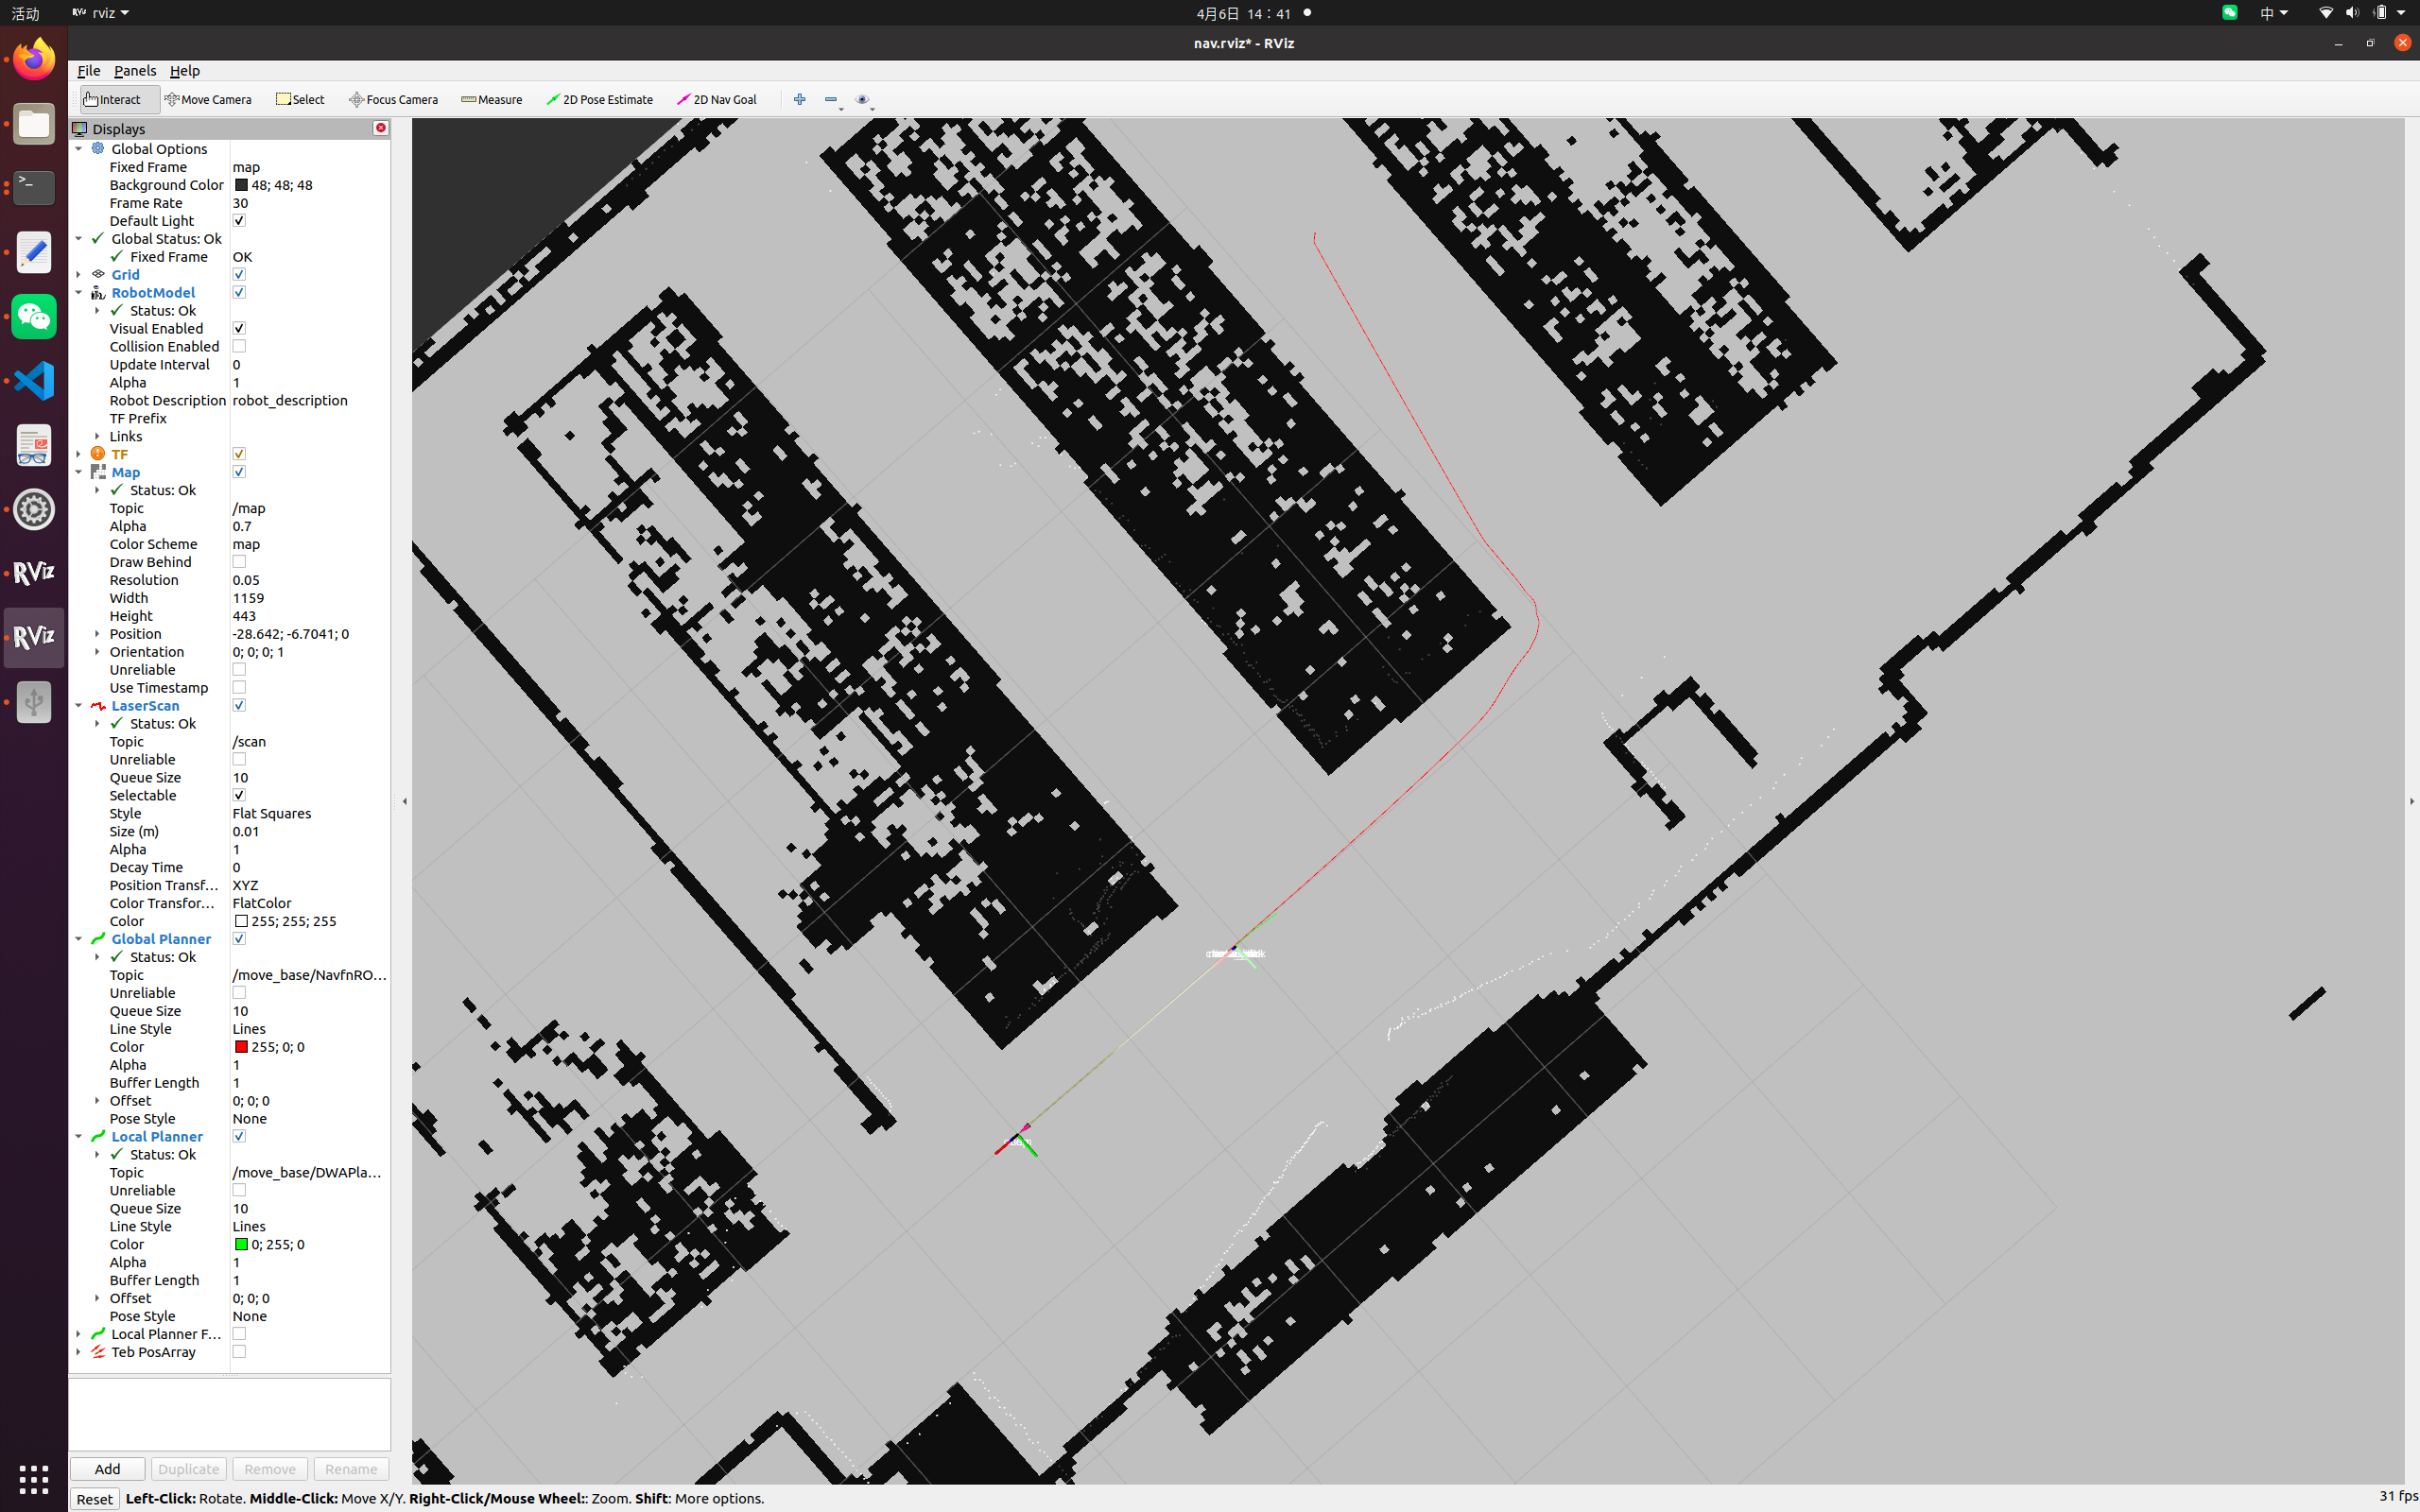
\includegraphics[width=\linewidth]{report_assets/exp2_lab_goal1.png}
\par\small Goal placement 1
\end{minipage}\hfill
\begin{minipage}[t]{0.32\textwidth}
\centering
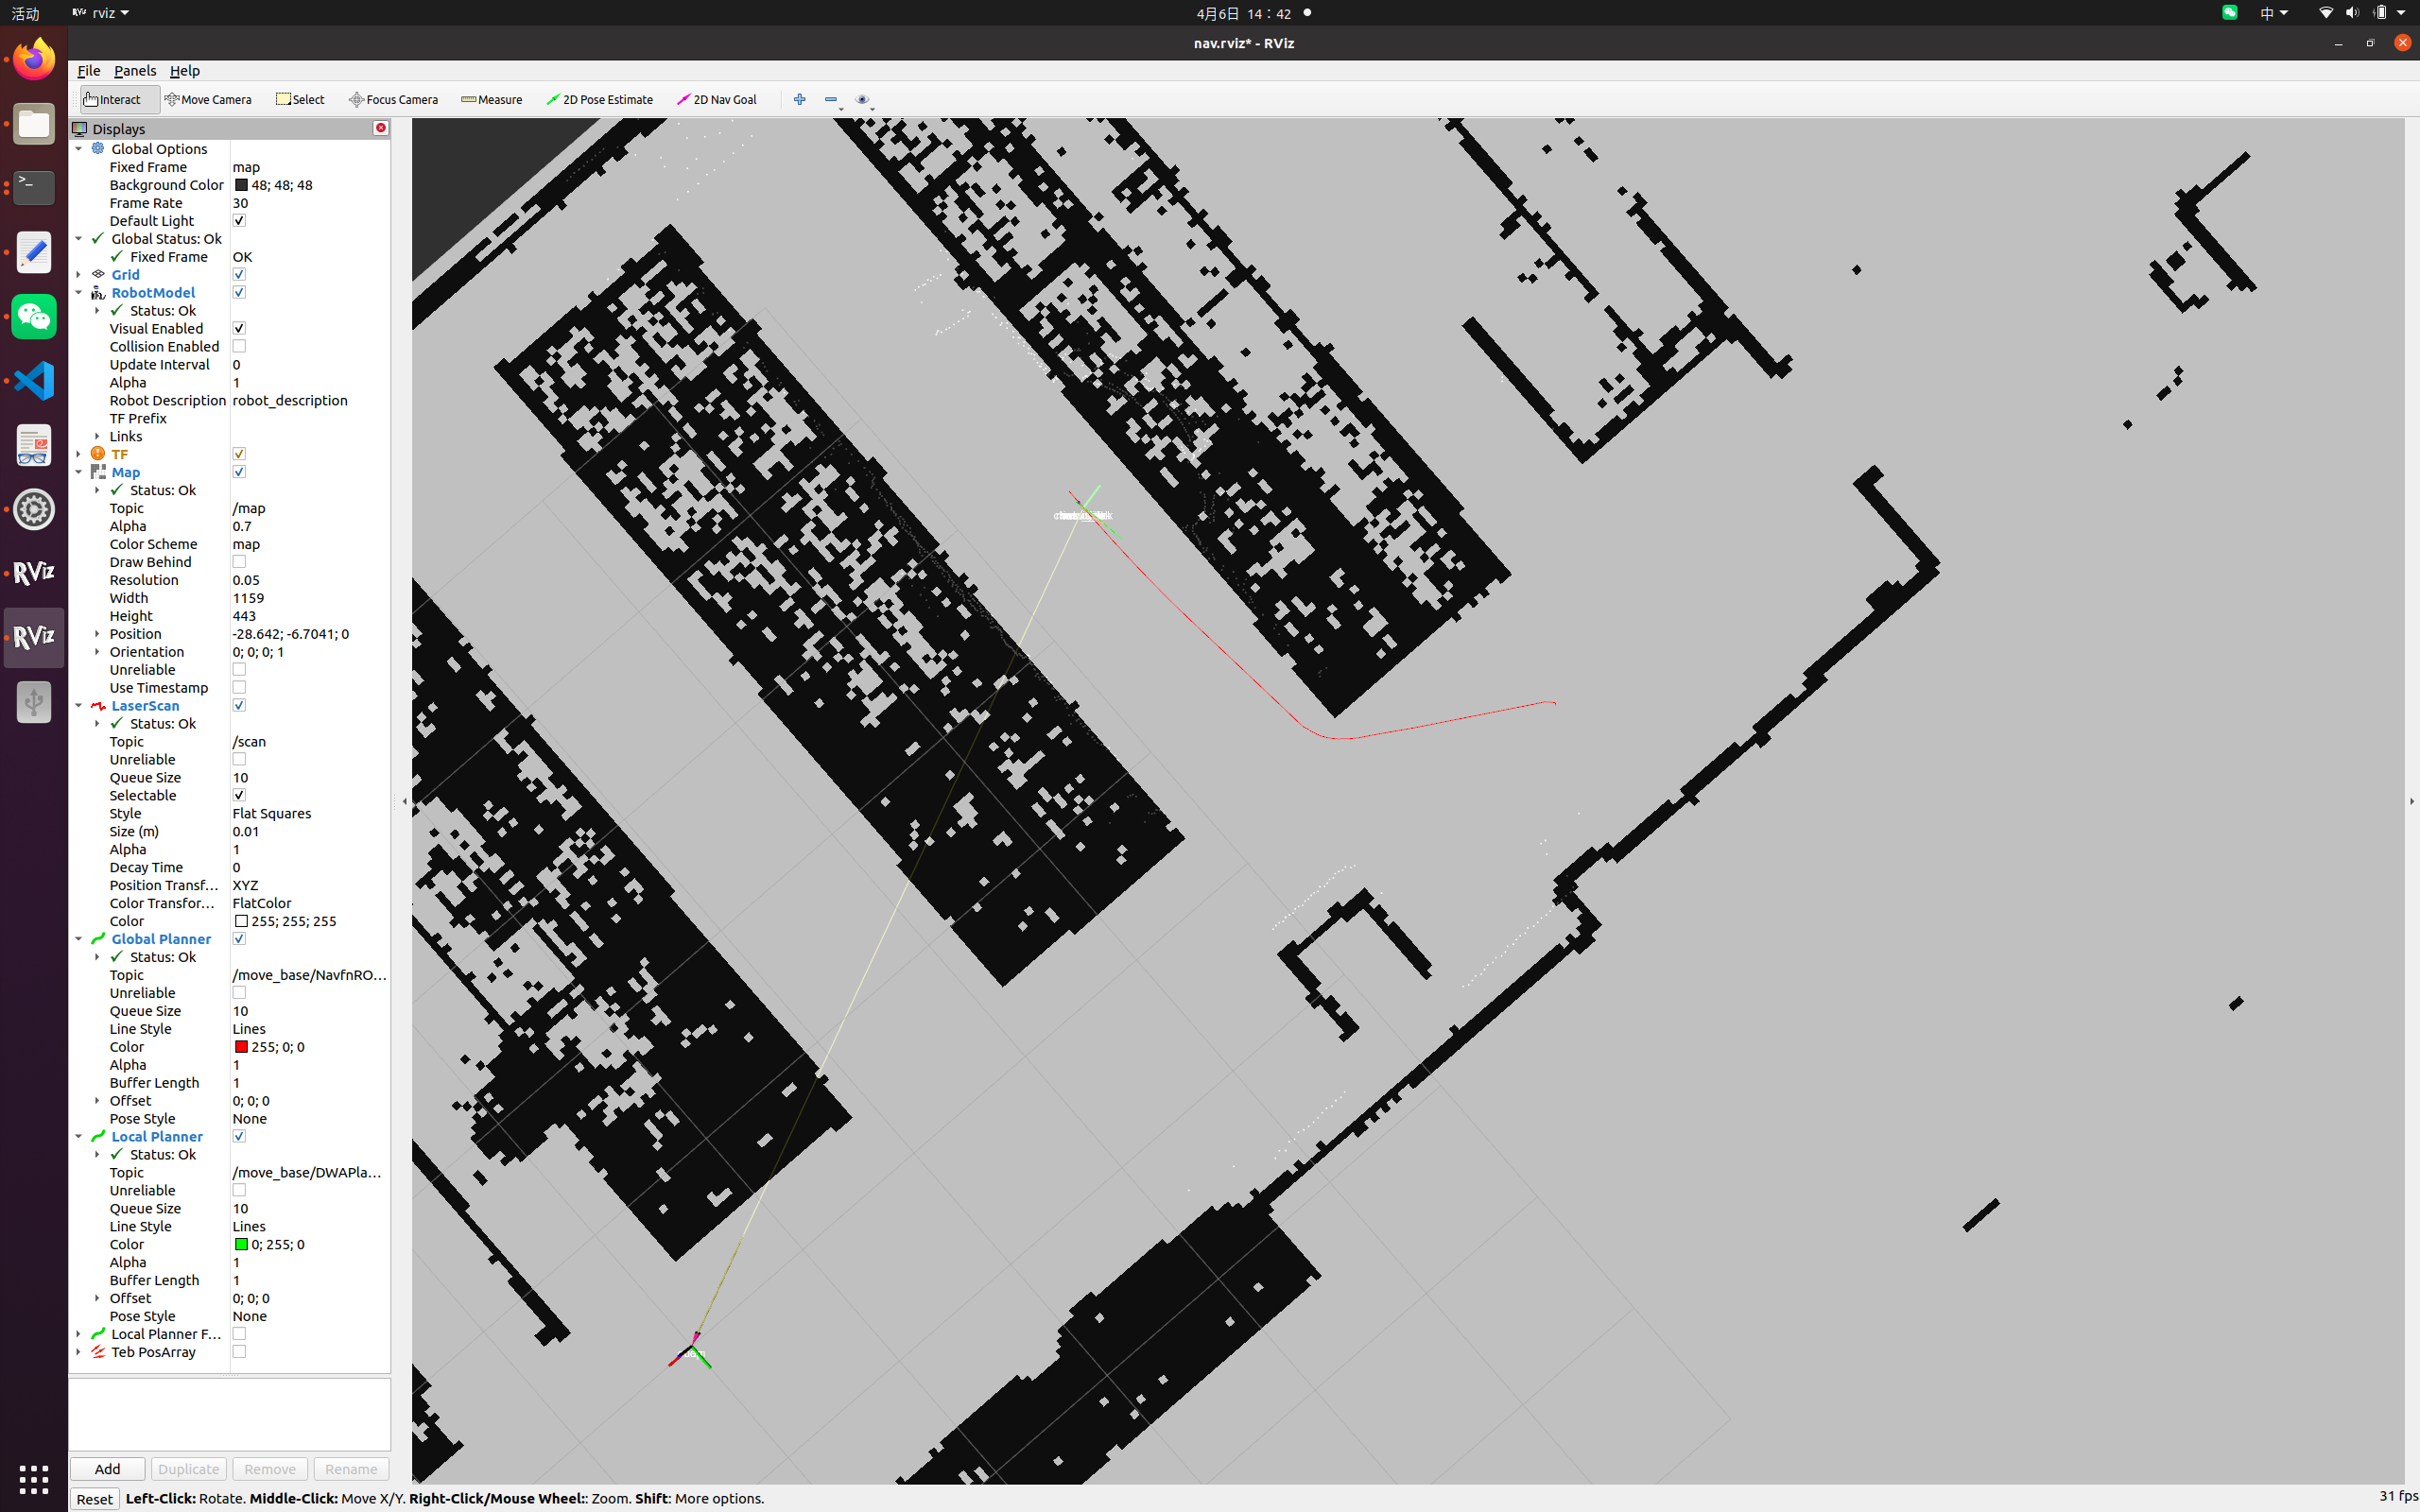
\includegraphics[width=\linewidth]{report_assets/exp2_lab_goal2.png}
\par\small Goal placement 2
\end{minipage}\hfill
\begin{minipage}[t]{0.32\textwidth}
\centering
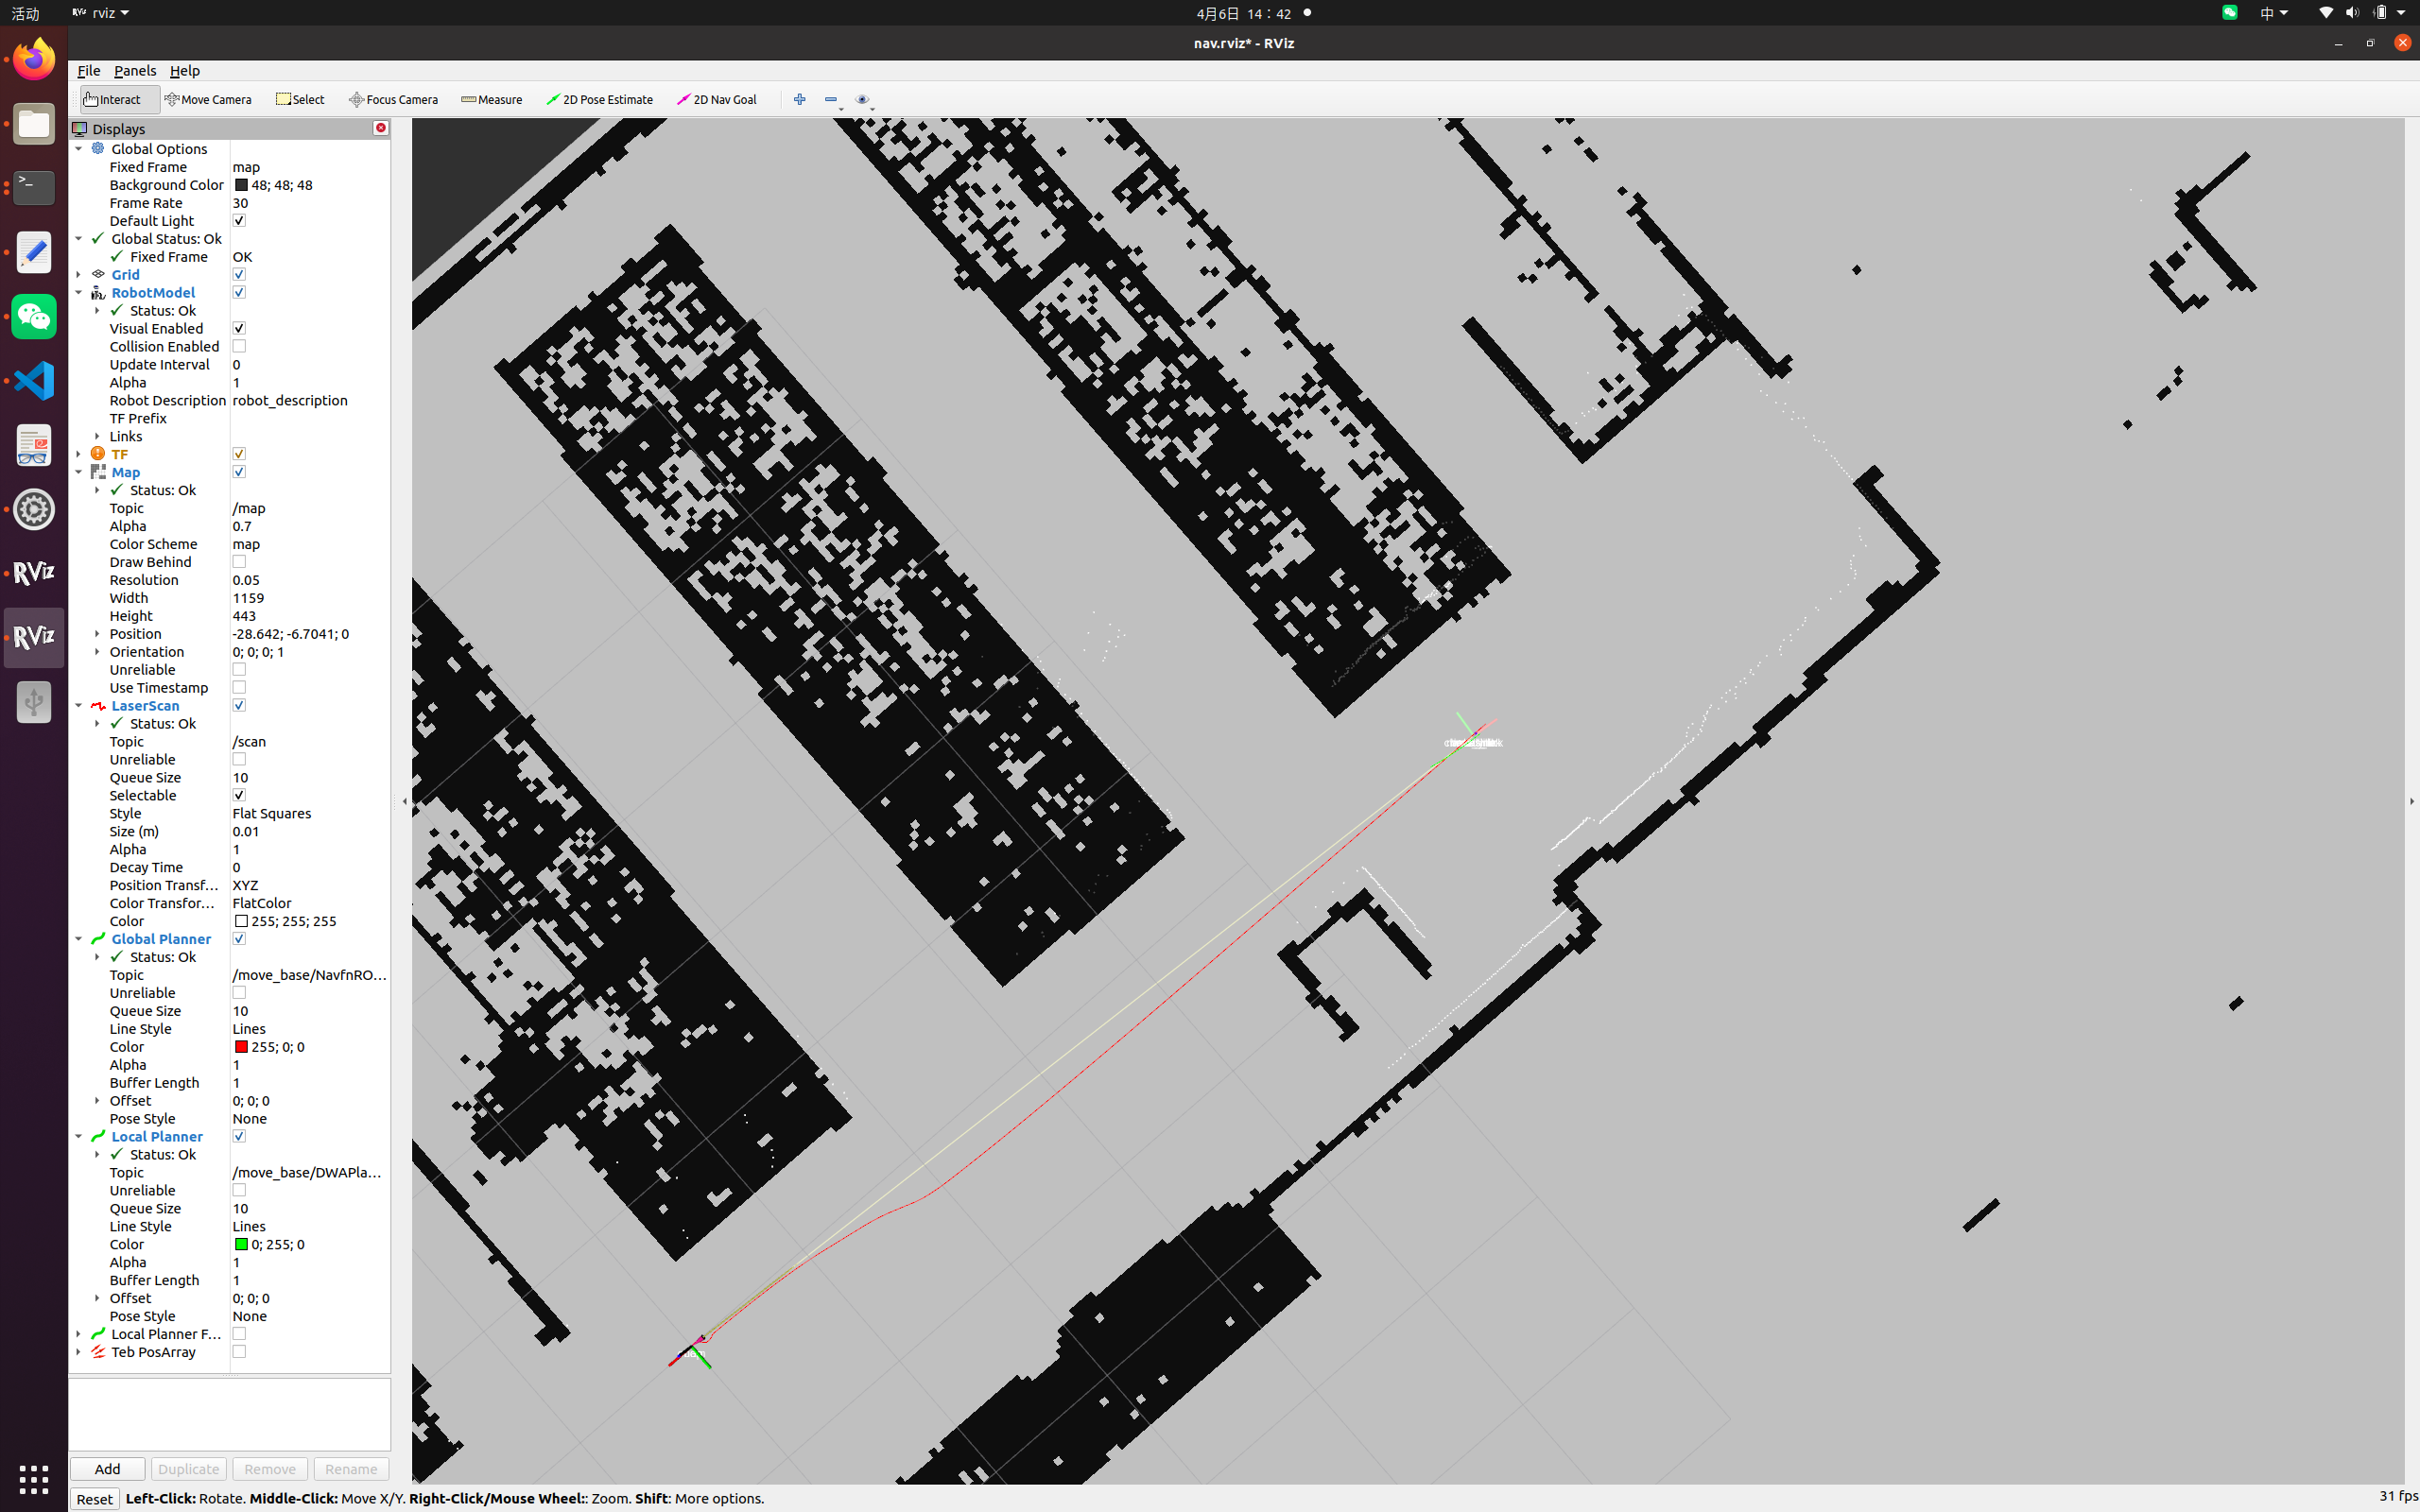
\includegraphics[width=\linewidth]{report_assets/exp2_lab_goal3.png}
\par\small Return segment design
\end{minipage}
\caption{Goal design for the indoor laboratory static-obstacle scenario. The route was first documented during the \texttt{exp2\_lab} pilot run and then reused for the repeated quantitative runs. The evaluator appends the robot start pose as a final return-to-start target, so the benchmark tests both forward route execution and return consistency.}
\label{fig:exp2-lab-route-design}
\end{figure}

The use of the \texttt{exp2\_lab} screenshots as a route-design record is important for report transparency. It shows that the later quantitative runs did not use different maps or different waypoint layouts for different algorithms. Instead, the same route structure was preserved and only the SLAM backend changed. This makes the indoor laboratory comparison a controlled navigation benchmark rather than a collection of loosely related demonstrations.

\subsubsection{Repeated Static-Obstacle Laboratory Benchmark}
The quantitative comparison for the laboratory scenario is therefore based on the averaged results from \texttt{exp3\_lab}, \texttt{exp4\_lab}, and \texttt{exp5\_lab}. Each of these runs used the same static-obstacle laboratory setup, the same map, the same route structure, and the same evaluator. Table~\ref{tab:online-summary-lab-avg} summarises the averaged results across the three repetitions.

\begin{table}[H]
\centering
\scriptsize
\caption{Average online results over the repeated indoor laboratory static-obstacle trials (\texttt{exp3\_lab}, \texttt{exp4\_lab}, and \texttt{exp5\_lab}).}
\label{tab:online-summary-lab-avg}
\setlength{\tabcolsep}{3pt}
\renewcommand{\arraystretch}{1.05}
\resizebox{\textwidth}{!}{%
\begin{tabular}{lrrrrrrrrrrr}
\toprule
Algorithm & Succ. rate & Avg time (s) & Avg total path (m) & Avg speed (m/s) & Min scan (m) & Near-coll. & Goal err. (m) & Return err. (m) & CPU (\%) & GPU (\%) \\
\midrule
LIO-SAM   & 1.000 & 95.851 & 19.539 & 0.204 & 0.678 & 0.000 & 0.232 & 0.233 & 13.491 & 31.508 \\
FAST-LIO  & 1.000 & 94.801 & 19.758 & 0.208 & 0.307 & 0.000 & 0.240 & 0.243 & 12.797 & 31.565 \\
Point-LIO & 1.000 & 86.351 & 19.401 & 0.225 & 0.316 & 0.000 & 0.239 & 0.238 & 12.856 & 31.153 \\
FASTER-LIO& 1.000 & 96.501 & 19.526 & 0.202 & 0.200 & 5.000 & 0.240 & 0.244 & 15.321 & 34.995 \\
\bottomrule
\end{tabular}
}
\end{table}

All four algorithms achieved a 100\% success rate over the repeated static-obstacle laboratory trials. This is already a meaningful result because it shows that, after the frame, cloud, and costmap integration issues were resolved, all four methods could complete the same route under the same navigation stack. The differences that remain are therefore not binary success-versus-failure differences, but system-level differences in efficiency, safety margin, and deployment cost.

The strongest performer in this repeated laboratory benchmark is Point-LIO. It achieved the shortest average completion time, the highest average speed, and the shortest average travelled path among the four methods, while still maintaining zero near-collision events. Its time variation across the three repeated runs is also very small, which indicates that the result is not a one-off best case but a stable pattern. In practical terms, this means that Point-LIO produced the most efficient route execution for the chosen laboratory task once its navigation bridge had been corrected to use the appropriate body-frame cloud.

FAST-LIO is the most balanced method in the same benchmark. It is slower than Point-LIO, but still clearly faster than LIO-SAM and FASTER-LIO on average. At the same time, it maintains zero near-collision events and the lowest average CPU consumption of the four methods. This balance is important from a deployment perspective. If a team values stable performance with low host-side resource demand and does not need the absolute shortest task time, FAST-LIO presents the strongest all-round trade-off in the repeated laboratory scenario.

LIO-SAM remains the most conservative method. Its average minimum obstacle distance of approximately \(0.678\,\mathrm{m}\) is far larger than that of the other three methods, and it also achieves the lowest average goal position error and the lowest return-to-start position error. However, this stronger safety margin and positional consistency come with a penalty in efficiency. LIO-SAM is noticeably slower than Point-LIO and somewhat slower than FAST-LIO on average. The laboratory benchmark therefore suggests that LIO-SAM is especially suitable when conservative clearance is more important than route completion speed.

FASTER-LIO performs the worst in the repeated indoor benchmark. Its average completion time is the longest, its average speed is the lowest, and, most importantly, it records an average of five near-collision events per run together with the smallest obstacle clearance among the four methods. This pattern is consistent across the three repeated experiments rather than being caused by one unusual run. The implication is not that FASTER-LIO is unusable, since it still completed all tasks successfully, but that its current integration in this navigation stack is more aggressive and less safe than the alternatives under the same static obstacle configuration.

The repeated laboratory benchmark also highlights an important methodological point: ``same planner parameters'' does not imply ``same navigation behaviour.'' The DWA parameters and costmap configuration were held constant across all three experiments, yet the observed task times, clearance margins, and near-collision patterns still differ substantially. This confirms one of the core engineering conclusions of the project: odometry quality, cloud type, frame conventions, and the suitability of the obstacle-observation topic can strongly reshape the behaviour of a fixed navigation backend. In other words, what is being compared here is not just four estimators in isolation, but four complete system outputs as they are consumed by a common navigation stack.

Another useful observation is that the repeated trials reduce the risk of over-interpreting one lucky run. Point-LIO is not judged superior merely because of a single good trajectory; it leads the group consistently across \texttt{exp3\_lab}, \texttt{exp4\_lab}, and \texttt{exp5\_lab}. Likewise, the weakness of FASTER-LIO is not a one-off anomaly because its obstacle clearance remains the worst across all three repetitions. This repeated-trial structure makes the laboratory result much more persuasive than the earlier single-run benchmark.

\subsubsection{Supplementary Dynamic-Obstacle Laboratory Demonstration}
In addition to the repeated static-obstacle benchmark, the project archive also contains an earlier indoor laboratory online experiment in which the obstacle layout was intentionally changed during the route. This archived result is represented by the \texttt{manual\_liosam} and \texttt{manual\_fastlio} summaries. Unlike the repeated \texttt{exp3\_lab}--\texttt{exp5\_lab} experiments, this test was not intended as the main fairness benchmark for all four algorithms. Instead, it serves a different purpose: to show that the integrated navigation system is able to react to changing local obstacles in real time rather than merely following a fixed route on a fixed map.

The route in this supplementary test consists of four manually captured goals, with the evaluator appending the start pose as a final return target. The obstacle arrangement was changed between route segments as follows:
\begin{enumerate}[leftmargin=2em]
    \item from the start pose to Goal 1, no additional obstacle was placed;
    \item from Goal 1 to Goal 2, obstacles were introduced into the workspace;
    \item from Goal 2 to Goal 3, the obstacle arrangement was changed again;
    \item from Goal 3 to the final manually set goal, the temporary obstacles were removed.
\end{enumerate}
This sequence is important because it tests whether the local costmap and scan-generation pipeline can support true online avoidance under changing obstacle conditions. In other words, it is not only a path-following test, but also a dynamic environment response test.

\begin{table}[H]
\centering
\small
\setlength{\tabcolsep}{5pt}
\caption{Supplementary indoor laboratory dynamic-obstacle online results archived for LIO-SAM and FAST-LIO.}
\label{tab:online-summary-lab-dynamic}
\begin{tabular}{lrr}
\toprule
Metric & LIO-SAM & FAST-LIO \\
\midrule
Goal count & 5 & 5 \\
Success count & 5 & 5 \\
Success rate & 1.000 & 1.000 \\
Total time (s) & 123.551 & 120.301 \\
Total path length (m) & 29.568 & 29.426 \\
Average speed (m/s) & 0.239 & 0.245 \\
Minimum scan distance (m) & 0.658 & 0.309 \\
Total recovery count & 0 & 0 \\
Total near-collision count & 0 & 0 \\
Average goal position error (m) & 0.237 & 0.241 \\
Return-to-start position error (m) & 0.240 & 0.243 \\
Average CPU (\%) & 12.559 & 12.448 \\
Average GPU (\%) & 13.164 & 15.475 \\
Average command linear std & 0.0286 & 0.0222 \\
Average command angular std & 0.1595 & 0.1045 \\
\bottomrule
\end{tabular}
\end{table}

Although only LIO-SAM and FAST-LIO were fully archived in this supplementary dynamic-obstacle run, the result is still valuable. Both methods achieved full task completion with zero recovery events and zero near-collision counts despite changes in obstacle placement between route segments. This means that the system was not merely replaying a static global path; it was able to keep updating obstacle observations and continue navigating successfully after the environment had been modified.

The comparison between the two methods in this dynamic test is also informative. FAST-LIO completed the route slightly faster and produced smoother command traces, while LIO-SAM maintained a much larger minimum scan distance, indicating a more conservative clearance policy. This pattern is consistent with later observations in the laboratory benchmark: FAST-LIO tends to be efficient and decisive, whereas LIO-SAM tends to preserve larger safety margins. For the dissertation, this dynamic-obstacle experiment therefore serves as supporting evidence that the system can perform real-time avoidance and that algorithm-dependent differences in local obstacle response are visible even when the high-level planner is fixed.

\subsubsection{Second Manual Laboratory Dynamic-Obstacle Benchmark}
To strengthen the online laboratory evidence beyond the earlier two-algorithm demonstration, a second manually supervised laboratory run was later archived under \texttt{lab\_manual2}. This experiment uses the same overall laboratory setting but extends the comparison to all four algorithms. As in the earlier manual run, the purpose is not to create a perfectly controlled repeated static benchmark, but to observe how each integrated navigation stack behaves when the operator monitors the route and local obstacle conditions in real time. The resulting benchmark is therefore especially useful for judging practical deployability: it reveals whether a backend can keep the common navigation stack stable while the robot moves through a realistic indoor route that is not reduced to a single frozen obstacle layout.

Table~\ref{tab:online-summary-lab-manual2} summarises the archived \texttt{lab\_manual2} results. Three methods, namely LIO-SAM, FAST-LIO, and FASTER-LIO, completed all five goals successfully. Point-LIO, by contrast, completed only the first goal and then failed the remaining sequence, resulting in a success rate of \(0.2\). The contrast is important because it confirms that the weaker online robustness of Point-LIO is not merely a one-off observation from the earlier manual benchmark. Under a second manually supervised laboratory run, the same broad pattern reappears: Point-LIO can begin the route, but the full navigation chain remains much less stable than that of the other three methods.

\begin{table}[H]
\centering
\scriptsize
\caption{Second manual indoor laboratory online benchmark (\texttt{lab\_manual2}) across all four algorithms.}
\label{tab:online-summary-lab-manual2}
\setlength{\tabcolsep}{3pt}
\renewcommand{\arraystretch}{1.05}
\resizebox{\textwidth}{!}{%
\begin{tabular}{lrrrrrrrrrrr}
\toprule
Algorithm & Succ. rate & Total time (s) & Total path (m) & Avg speed (m/s) & Min scan (m) & Near-coll. & Goal err. (m) & Return err. (m) & CPU (\%) & GPU (\%) \\
\midrule
LIO-SAM    & 1.000 & 133.301 & 30.045 & 0.225 & 0.678 & 0 & 0.233 & 0.223 & 12.854 & 12.359 \\
FAST-LIO   & 1.000 & 132.351 & 30.095 & 0.227 & 0.319 & 0 & 0.242 & 0.245 & 12.415 & 12.443 \\
Point-LIO  & 0.200 & 69.907  & 15.286 & 0.219 & 0.357 & 0 & 3.278 & 7.285 & 11.725 & 10.676 \\
FASTER-LIO & 1.000 & 129.701 & 29.705 & 0.229 & 0.200 & 15 & 0.243 & 0.234 & 15.349 & 17.383 \\
\bottomrule
\end{tabular}
}
\end{table}

Among the fully successful methods, FASTER-LIO is the fastest in terms of total completion time and total travelled path. However, it again reaches this result by using the smallest obstacle clearance and by accumulating 15 near-collision events. This is highly consistent with the earlier laboratory observations and reinforces the interpretation that FASTER-LIO is operational but aggressive in the current navigation integration. It offers strong task efficiency, yet it does so at the cost of the weakest safety margin in the group.

FAST-LIO and LIO-SAM show a more deployment-friendly balance. FAST-LIO completes the full route with zero near-collision events, slightly shorter total time than LIO-SAM, and comparatively low CPU/GPU load. LIO-SAM is slightly slower, but it retains by far the largest minimum obstacle distance and again achieves the smallest average goal position error. In other words, the second manual laboratory benchmark preserves the same system-level distinction already visible elsewhere in the report: FAST-LIO is the most balanced and efficient option, whereas LIO-SAM is the most conservative and accuracy-oriented option.

Point-LIO is the clear outlier in this four-way manual benchmark. The per-goal archive shows that it successfully reaches the first goal, but then fails on the second segment and never regains stable progress for the remaining route. The result is not simply a modest slowdown; the average goal position error rises above \(3.2\,\mathrm{m}\), and the final return-to-start error exceeds \(7.2\,\mathrm{m}\). This supports the broader project conclusion that Point-LIO, in the current integration, is not primarily limited by nominal peak speed or low resource use, but by insufficient online robustness once the full navigation chain is stressed over multiple route segments.

Taken together, the two manually supervised laboratory benchmarks now serve different but complementary roles in the report. The earlier \texttt{manual} archive demonstrates that the system can react to changing obstacle layouts in real time using at least two fully integrated backends. The newer \texttt{lab\_manual2} archive extends this insight into a four-algorithm comparison and makes the separation between the methods more explicit: LIO-SAM and FAST-LIO remain reliable, FASTER-LIO is fast but aggressive, and Point-LIO remains the least stable in online navigation despite parameter alignment efforts. This is a valuable systems conclusion because it shows that online navigation quality depends on more than raw localisation accuracy alone; it also depends on whether the backend provides odometry and obstacle observations in a form that the common planner can consume robustly over an entire task.

\subsubsection{Fixed Human-Interference Laboratory Benchmark}
An additional laboratory benchmark was later archived under \texttt{lab/lab\_moving\_obs}. The most complete four-algorithm comparison currently available in that folder is the first archived run, denoted here as \texttt{exp1}. In this experiment, the robot was assigned a single forward navigation goal while the operator deliberately stepped into the robot's route five times, each time leaving enough free space for the robot to re-route rather than fully blocking the path. Because the number of human interventions was controlled by the experimental protocol itself, the comparison here focuses on aggregate navigation outcomes instead of automatically counted obstruction events. The most relevant quantities are therefore task success, total traversal time, total travelled path length, average speed, safety margin, stop behaviour, final goal error, and computational load.

Table~\ref{tab:online-summary-lab-human} summarises the archived four-algorithm comparison for \texttt{exp1}. Three methods, namely LIO-SAM, FAST-LIO, and FASTER-LIO, reached the goal successfully. Point-LIO did not. The contrast is strong enough that the result can be used as a practical robustness benchmark even without repeated trials: all four methods faced the same map, the same goal, the same planner, and the same manually imposed five-intervention obstacle protocol.

\begin{table}[H]
\centering
\scriptsize
\caption{Fixed human-interference indoor laboratory benchmark (\texttt{lab\_moving\_obs}, \texttt{exp1}) across all four algorithms. Each run used the same single-goal route and the same five planned human interventions.}
\label{tab:online-summary-lab-human}
\setlength{\tabcolsep}{3pt}
\renewcommand{\arraystretch}{1.05}
\resizebox{\textwidth}{!}{%
\begin{tabular}{lrrrrrrrrrrr}
\toprule
Algorithm & Succ. rate & Total time (s) & Total path (m) & Avg speed (m/s) & Min scan (m) & Recovery & Near-coll. & Goal err. (m) & Stop time (s) & CPU (\%) & GPU (\%) \\
\midrule
LIO-SAM    & 1.000 & 40.700 & 9.673 & 0.238 & 0.675 & 0 & 0 & 0.236 & 0.00   & 4.215 & 12.808 \\
FAST-LIO   & 1.000 & 40.850 & 9.740 & 0.238 & 0.312 & 0 & 0 & 0.250 & 0.300  & 3.001 & 11.410 \\
Point-LIO  & 0.000 & 150.081 & 9.243 & 0.062 & 0.318 & 2 & 0 & 3.668 & 117.700& 3.611 & 15.913 \\
FASTER-LIO & 1.000 & 41.150 & 9.717 & 0.236 & 0.200 & 0 & 0 & 0.240 & 0.200  & 5.140 & 13.641 \\
\bottomrule
\end{tabular}
}
\end{table}

The result adds an important practical layer to the laboratory evaluation. Under repeated human interference, LIO-SAM delivered the strongest overall performance. It achieved the shortest completion time, the shortest effective route among the successful methods, zero recovery events, zero near-collision events, and by far the largest minimum obstacle distance. In other words, it remained both successful and conservative under a route condition that repeatedly forced the robot to react to a person entering its path.

FAST-LIO remained very competitive. Its completion time was only marginally slower than that of LIO-SAM, and it used the lowest CPU and GPU resources among the successful methods. This makes FAST-LIO the most resource-efficient successful solution in the benchmark. The trade-off is that its minimum obstacle distance was much smaller than that of LIO-SAM, indicating a more decisive but less conservative response to a person standing near the route.

FASTER-LIO also completed the task successfully, but it again showed the most aggressive safety profile. Its minimum scan distance dropped to approximately \(0.20\,\mathrm{m}\), which is substantially smaller than the clearance maintained by both LIO-SAM and FAST-LIO. The benchmark therefore reinforces an interpretation that has appeared elsewhere in the report: FASTER-LIO can complete navigation tasks efficiently, but it tends to do so with the weakest obstacle clearance margin in the current integration.

Point-LIO is the clear outlier. It failed to reach the goal within the timeout, triggered two recovery events, and accumulated more than \(117\,\mathrm{s}\) of stop time in a run lasting about \(150\,\mathrm{s}\). This means that the robot spent most of the experiment effectively stalled rather than progressing toward the goal. The final goal error of approximately \(3.67\,\mathrm{m}\) confirms that this was not a near miss but a substantial task failure. The significance of this result is not merely that Point-LIO can be slower; rather, it shows that under repeated human interference the integrated Point-LIO navigation chain can lose practical task robustness altogether.

This fixed human-interference benchmark is especially useful because it bridges the gap between the repeated static-obstacle laboratory test and the earlier manual obstacle-rearrangement runs. The static benchmark measures repeatable route execution under a frozen layout. The earlier manual benchmark showed that the system could still react when obstacle placement changed between route segments. By contrast, the \texttt{lab\_moving\_obs} experiment stresses repeated person-induced route interruption during a single live goal execution. The resulting picture is therefore richer: LIO-SAM appears to be the strongest option when conservative human-aware clearance matters most; FAST-LIO remains the most efficient and deployment-friendly successful backend; FASTER-LIO remains workable but aggressive; and Point-LIO remains the least stable in the face of sustained online disturbance.

\subsection{Outdoor Scenario}
The outdoor scenario is included in the final experimental design because it stresses different properties from the laboratory map. In a more open environment, the relative importance of obstacle proximity, long-range odometric consistency, and route completion time changes. The final report should therefore compare all four algorithms again under the outdoor map rather than extrapolating directly from the laboratory baseline.

From an engineering perspective, the outdoor scenario is expected to favour algorithms that remain stable with weaker geometric constraints and less frequent close-range structural returns. The final judgement, however, should be made only after the four standardised summary files are archived for this scenario.

\subsection{Corridor Scenario}
The corridor scenario is included because it places the strongest demand on local costmap responsiveness, scan generation quality, and narrow-space behaviour. Unlike the indoor laboratory dynamic-obstacle test, the \texttt{corridor2} route is intentionally configured as a no-obstacle navigation baseline. Its purpose is to evaluate how each SLAM backend behaves when the robot traverses a long, visually constrained corridor without the additional complication of manually rearranged obstacles. This makes the corridor test complementary to the indoor laboratory experiments: the laboratory scenario demonstrates real-time reaction to changing local obstacles, while the corridor scenario demonstrates how well each method supports clean route execution in a narrow static passage.

\subsubsection{No-Obstacle Corridor Benchmark}
The archived \texttt{corridor2} experiment uses a simple forward-and-return route in a long corridor environment. Figure~\ref{fig:corridor2-route-design} shows screenshots captured during the route setup and execution. In practice, the robot is first sent toward a corridor-end goal, after which the evaluator appends the robot start pose as the return target. No temporary obstacle is added between route segments. The benchmark therefore isolates the baseline interaction between odometry quality, map consistency, scan generation, and DWA control inside a narrow passage where walls remain continuously visible and local clearance is always relevant.

\begin{figure}[H]
\centering
\begin{minipage}[t]{0.48\textwidth}
\centering
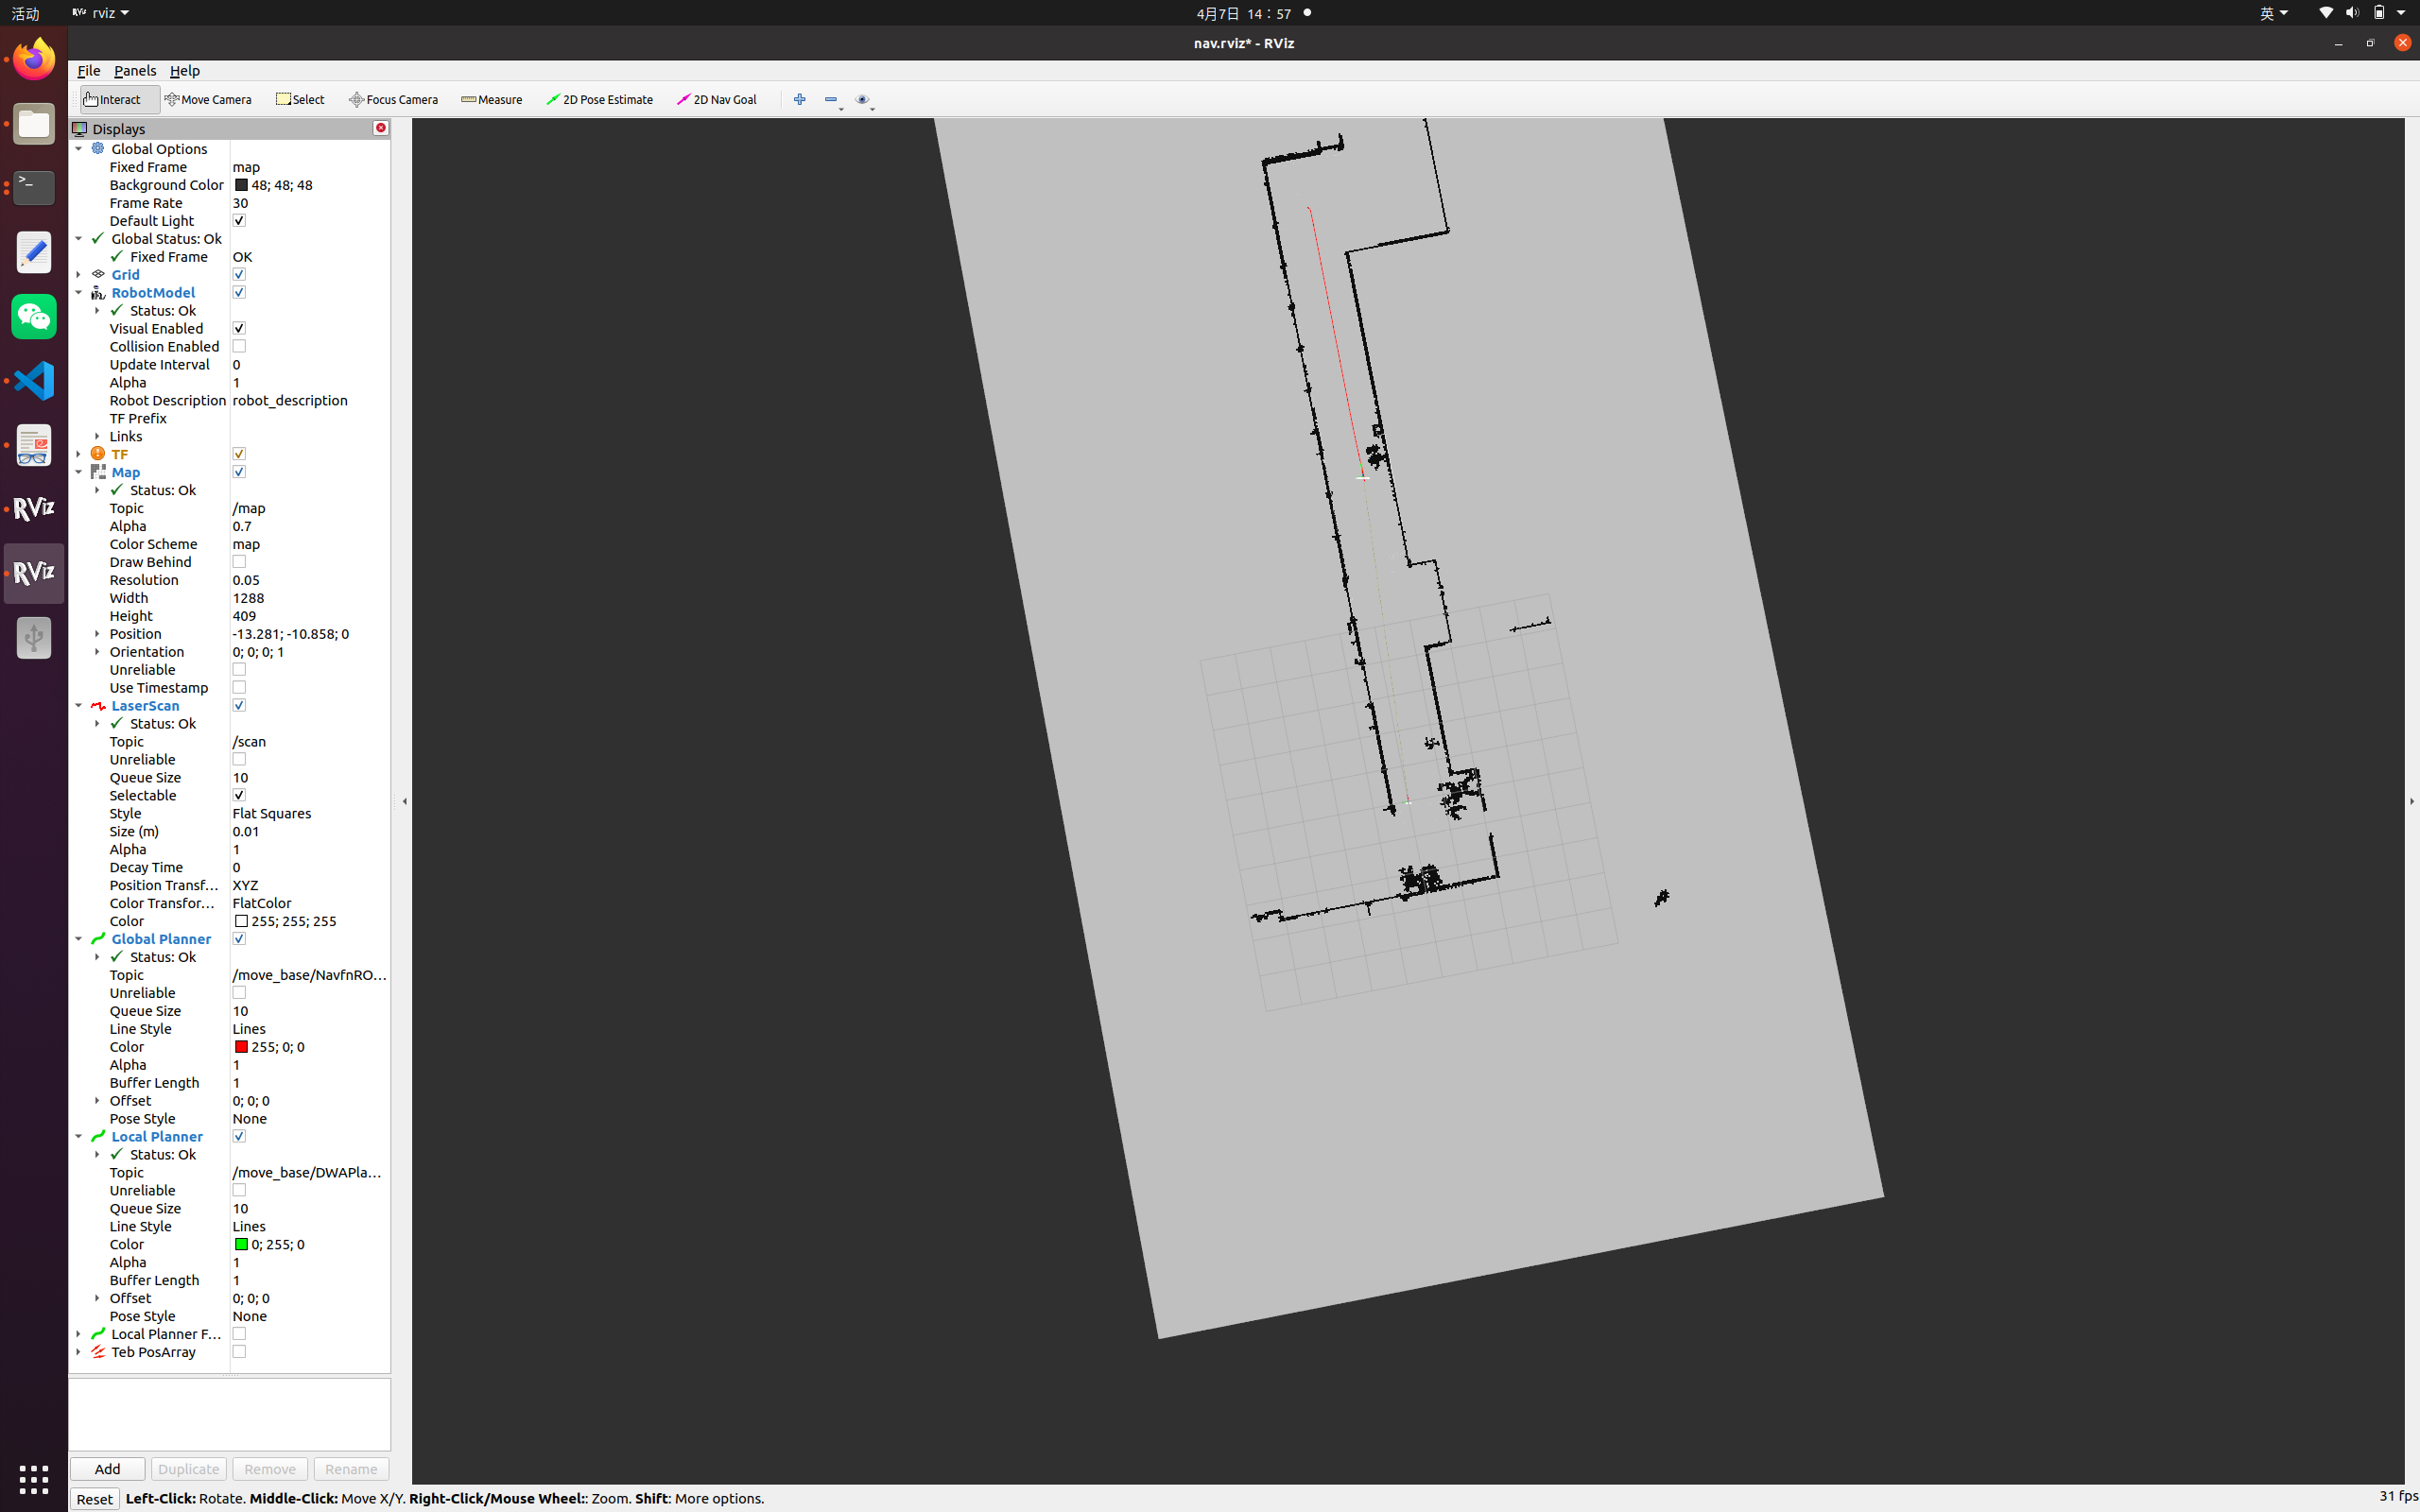
\includegraphics[width=\linewidth]{report_assets/corridor2_route1.png}
\par\small Forward corridor route
\end{minipage}\hfill
\begin{minipage}[t]{0.48\textwidth}
\centering
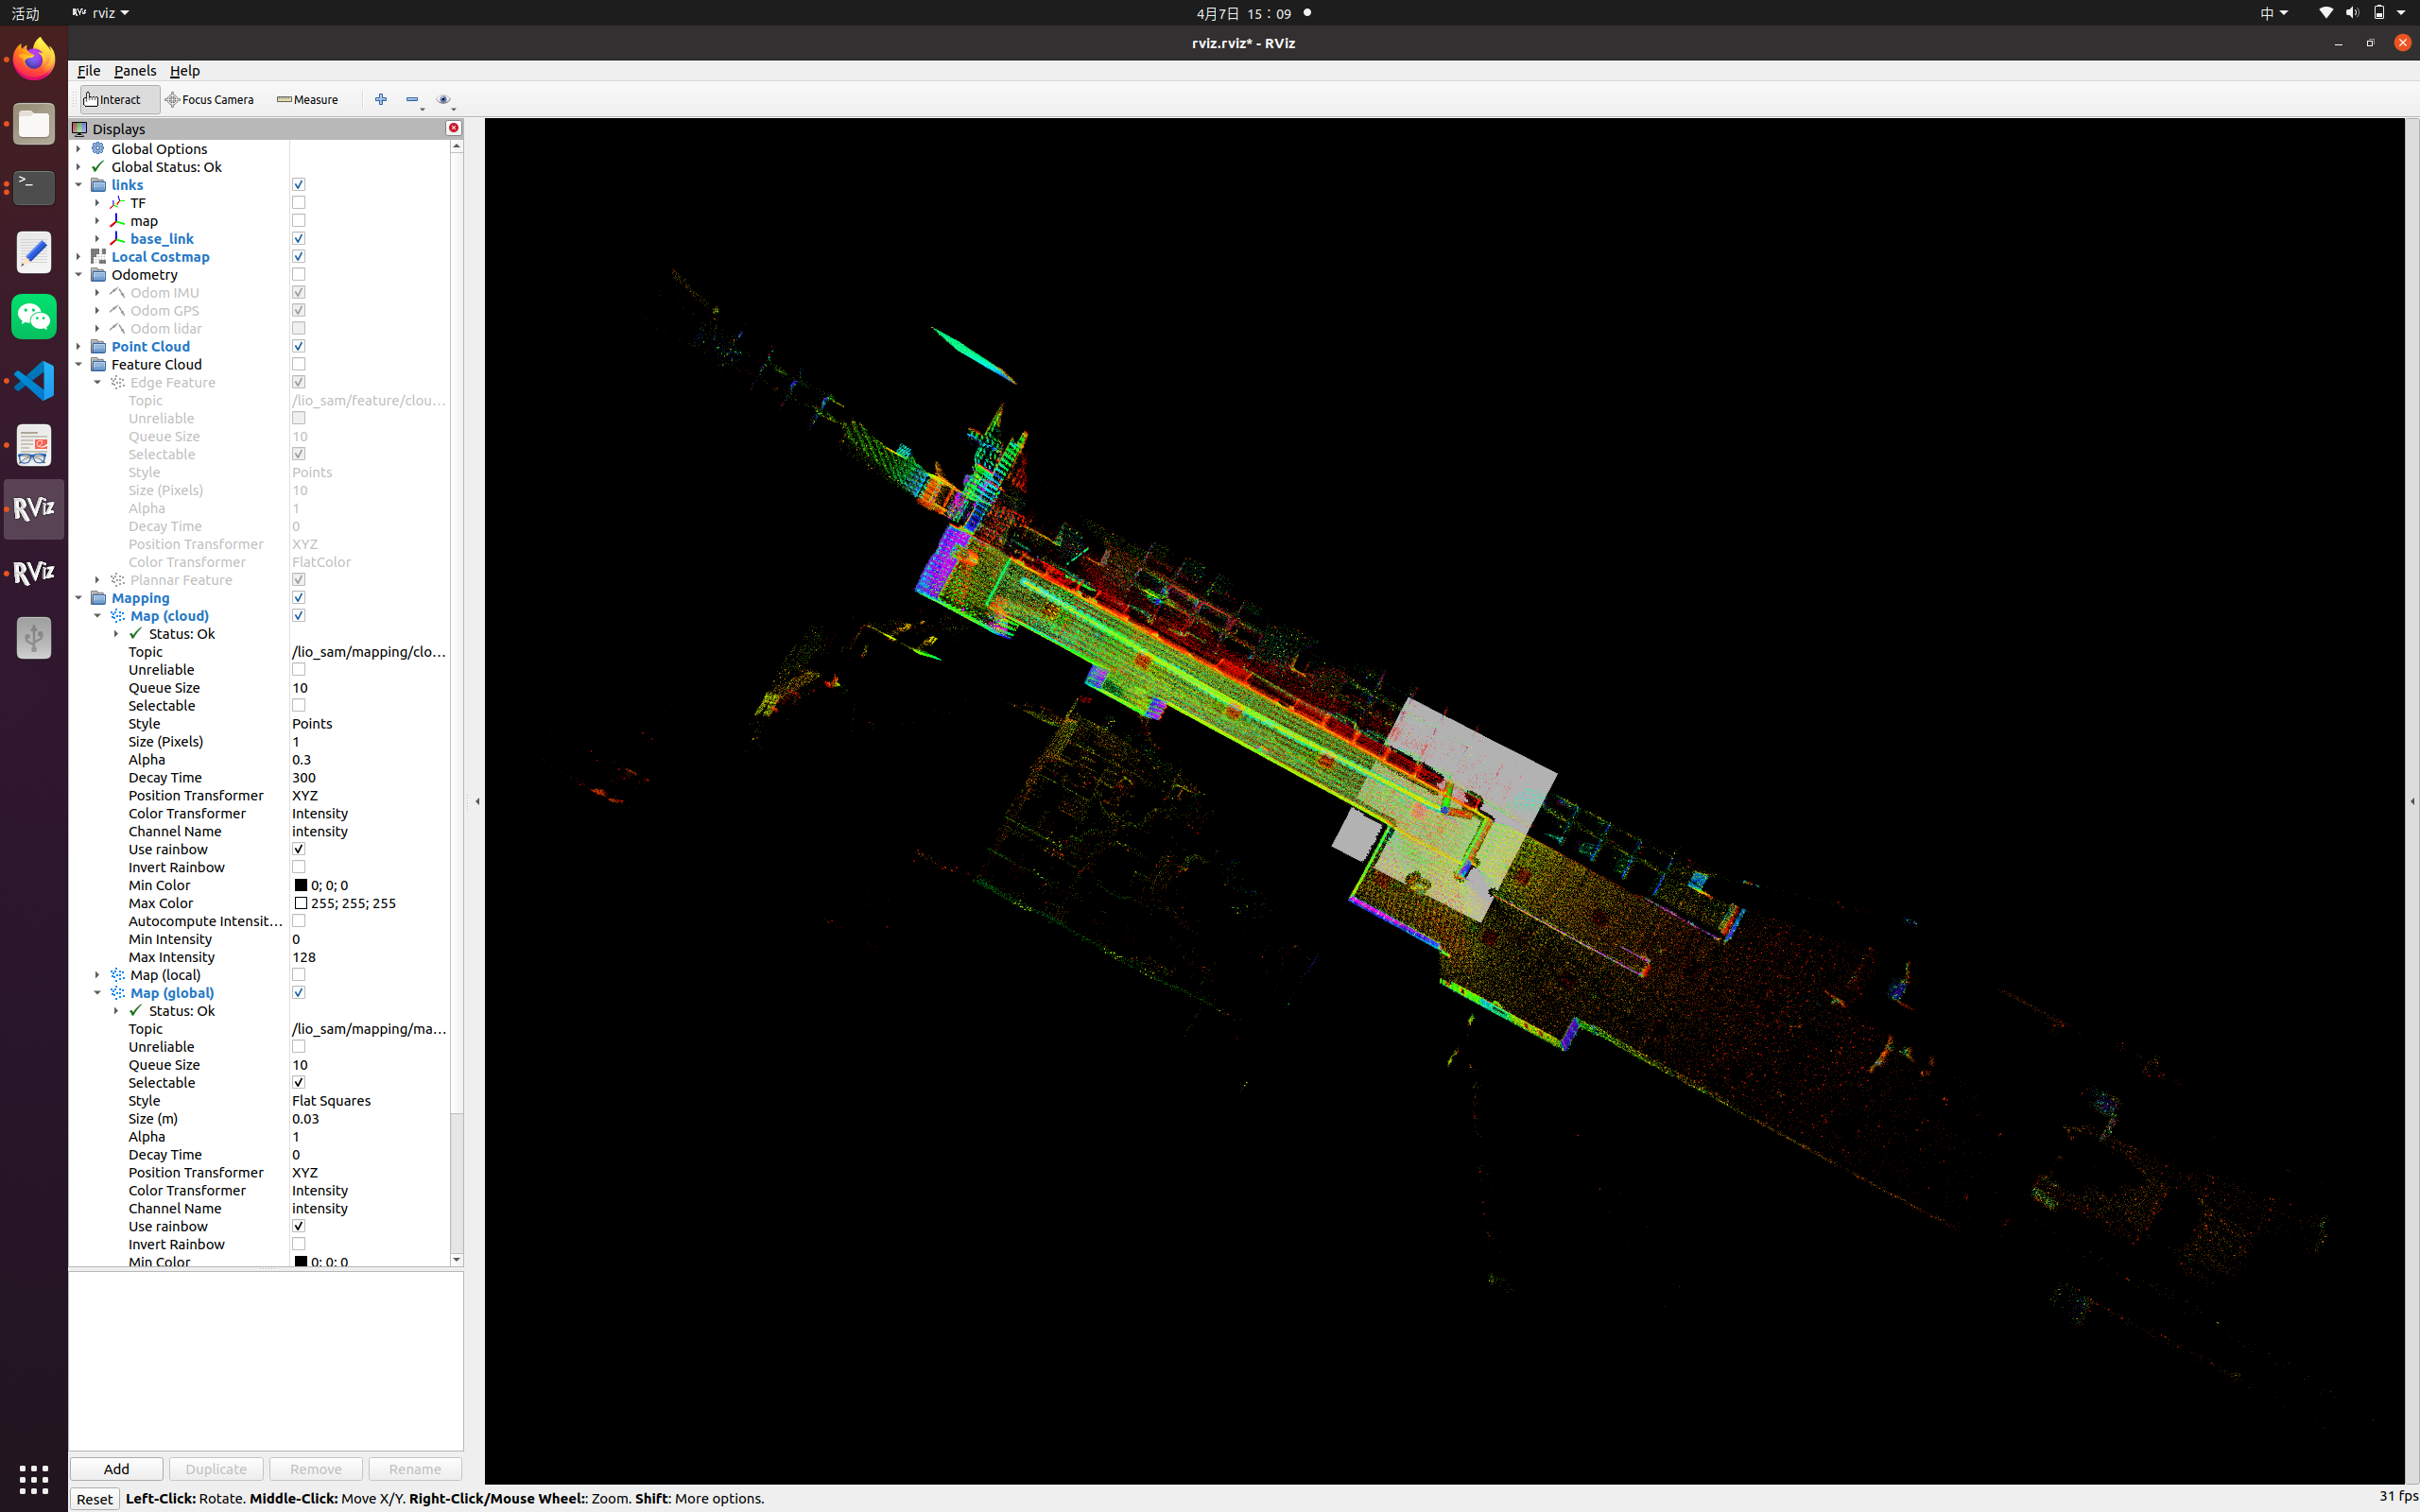
\includegraphics[width=\linewidth]{report_assets/corridor2_route2.png}
\par\small Return-to-start segment
\end{minipage}
\caption{Route design for the \texttt{corridor2} no-obstacle corridor benchmark. The robot first travels to the corridor-end goal and then returns to the start pose. No temporary obstacle is introduced during this experiment, making it a clean narrow-passage baseline that complements the dynamic-obstacle indoor laboratory demonstration.}
\label{fig:corridor2-route-design}
\end{figure}

At the time of writing, the fully archived four-algorithm corridor comparison is available for \texttt{exp1\_corridor2}. Additional repeated corridor runs have so far been archived only for LIO-SAM, so the present four-way comparison is best understood as a first corridor baseline rather than a repeated-trial average. Even so, the result is useful because all four algorithms are evaluated on the same map, the same route, and the same evaluator configuration. Table~\ref{tab:online-summary-corridor-exp1} summarises the benchmark.

\begin{table}[H]
\centering
\scriptsize
\caption{Online results for the no-obstacle corridor benchmark (\texttt{exp1\_corridor2}).}
\label{tab:online-summary-corridor-exp1}
\setlength{\tabcolsep}{3pt}
\renewcommand{\arraystretch}{1.05}
\resizebox{\textwidth}{!}{%
\begin{tabular}{lrrrrrrrrrr}
\toprule
Algorithm & Succ. rate & Total time (s) & Total path (m) & Avg speed (m/s) & Min scan (m) & Near-coll. & Goal err. (m) & Return err. (m) & CPU (\%) & GPU (\%) \\
\midrule
LIO-SAM    & 1.000 & 143.900 & 34.145 & 0.237 & 0.680 & 0 & 0.242 & 0.243 & 13.262 & 31.043 \\
FAST-LIO   & 1.000 & 143.000 & 34.185 & 0.239 & 0.344 & 0 & 0.238 & 0.235 & 3.100  & 31.892 \\
Point-LIO  & 1.000 & 146.800 & 34.161 & 0.233 & 0.379 & 0 & 0.246 & 0.248 & 3.224  & 30.196 \\
FASTER-LIO & 1.000 & 144.433 & 34.084 & 0.236 & 0.410 & 0 & 0.241 & 0.237 & 5.569  & 36.261 \\
\bottomrule
\end{tabular}
}
\end{table}

All four algorithms completed the corridor task successfully, with zero recovery events and zero near-collision events. This is an encouraging result because it shows that, once the cloud-to-scan bridge was corrected for each backend, the common navigation stack could execute a narrow-passage route reliably across all four SLAM methods. The comparison is therefore no longer about whether the system works at all, but about how efficiently and how conservatively each backend supports the same route.

FAST-LIO delivered the strongest overall corridor performance in this archived run. It achieved the shortest completion time, the highest average speed, and the smallest goal and return position errors, while also keeping CPU consumption very low. In practical terms, this means that FAST-LIO offered the best efficiency-accuracy trade-off in the no-obstacle corridor baseline. Its minimum obstacle distance is the smallest of the four methods, which indicates a more aggressive path selection, but in this particular experiment the trajectory remained safe and did not trigger any near-collision event.

LIO-SAM behaved very differently. Its completion time is only slightly slower than that of FAST-LIO, yet it maintains by far the largest minimum obstacle distance, approximately \(0.680\,\mathrm{m}\). This makes LIO-SAM the most conservative method in the corridor scenario, consistent with earlier observations in the indoor laboratory experiments. The price of this larger safety margin is a much higher CPU requirement. The corridor result therefore reinforces the interpretation that LIO-SAM is especially attractive when robust clearance is valued more highly than raw computational efficiency.

FASTER-LIO occupies a middle position in this corridor benchmark. It is slightly slower than FAST-LIO and slightly faster than Point-LIO, while preserving a larger clearance than FAST-LIO and Point-LIO. However, this moderate performance comes at the cost of the highest GPU load among the four methods. In other words, FASTER-LIO does not fail in the corridor environment, but it also does not dominate any of the key metrics once deployment cost is taken into account.

Point-LIO is the weakest method in this particular no-obstacle corridor run. It records the longest completion time, the lowest average speed, and the largest position errors, even though its CPU and GPU requirements remain modest. This result should not be over-generalised, because the corridor archive is not yet as complete as the repeated indoor laboratory benchmark. Nevertheless, within the currently archived four-way corridor comparison, Point-LIO is the least convincing option.

This corridor benchmark is important for the overall dissertation argument because it complements the indoor dynamic-obstacle demonstration in a meaningful way. The dynamic indoor test shows that the system can react to changing obstacle placement in real time. The corridor benchmark, by contrast, removes those manually introduced obstacle changes and focuses on baseline route execution inside a spatially constrained passage. Together, the two experiments show that the final navigation stack is not limited to a single favourable setup: it can both respond to changing local obstacles and perform stable narrow-passage navigation when the route is geometrically demanding but obstacle-free.

\subsubsection{Human-Interference Corridor Benchmark}
The local archive also contains a more demanding corridor experiment under \texttt{corridor2\_moving\_obs}, in which the operator repeatedly stepped into the robot's intended route while still leaving enough free space for a safe bypass. Compared with the no-obstacle corridor benchmark, this setup is much harsher because it combines narrow geometry with repeated live disturbances along the route. The benchmark is therefore useful as a stress test of corridor robustness rather than as a pure path-following trial.

The most informative archived four-algorithm comparison for this setting is \texttt{exp2}. Table~\ref{tab:online-summary-corridor-human} summarises the results. Unlike the no-obstacle corridor baseline, this run does not show universal success. Only LIO-SAM and FASTER-LIO reached the corridor-end goal successfully. FAST-LIO and Point-LIO both failed before convergence, making this experiment a strong indicator of which navigation backends remain operational when repeated human interference is introduced in a narrow corridor.

\begin{table}[H]
\centering
\scriptsize
\caption{Online results for the human-interference corridor benchmark (\texttt{corridor2\_moving\_obs}, \texttt{exp2}).}
\label{tab:online-summary-corridor-human}
\setlength{\tabcolsep}{3pt}
\renewcommand{\arraystretch}{1.05}
\resizebox{\textwidth}{!}{%
\begin{tabular}{lrrrrrrrrrr}
\toprule
Algorithm & Succ. rate & Total time (s) & Total path (m) & Avg speed (m/s) & Min scan (m) & Recovery & Near-coll. & Goal err. (m) & CPU (\%) & GPU (\%) \\
\midrule
LIO-SAM    & 1.000 & 73.000 & 17.323 & 0.237 & 0.677 & 0 & 0 & 0.235 & 13.855 & 11.620 \\
FAST-LIO   & 0.000 & 43.605 & 10.351 & 0.237 & 0.320 & 0 & 0 & 6.905 & 13.240 & 12.786 \\
Point-LIO  & 0.000 & 53.020 & 8.230  & 0.155 & 0.338 & 2 & 0 & 11.788 & 12.767 & 12.000 \\
FASTER-LIO & 1.000 & 72.300 & 17.288 & 0.239 & 0.205 & 0 & 2 & 0.249 & 15.531 & 15.141 \\
\bottomrule
\end{tabular}
}
\end{table}

LIO-SAM delivered the strongest overall corridor result under human interference. It completed the task successfully, preserved the largest obstacle clearance by a very large margin, and still maintained competitive traversal time and speed. This is important because it shows that the conservative behaviour previously observed in the laboratory scenario remains advantageous in a much tighter environment. The result is not simply that LIO-SAM is slower but safer; in this run it is both safe and fully successful.

FASTER-LIO was also able to complete the task, and its total completion time was slightly shorter than that of LIO-SAM. However, this apparent efficiency came with a much more aggressive safety profile. Its minimum scan distance dropped to approximately \(0.205\,\mathrm{m}\), and it accumulated two near-collision events. In practical terms, FASTER-LIO reached the goal, but it did so with the weakest clearance margin among the successful methods. This keeps the interpretation consistent with earlier laboratory results: FASTER-LIO can be effective, but in the current navigation stack it remains more aggressive than desirable in safety-critical corridor motion.

FAST-LIO and Point-LIO both failed in this benchmark, but their failure modes are different. FAST-LIO failed conservatively. It maintained zero recoveries and zero near-collision events, and its average speed remained close to its successful baselines elsewhere, yet it still did not converge to the goal and finished with a large final position error of approximately \(6.9\,\mathrm{m}\). This suggests that in the corridor human-interference scenario, FAST-LIO is not losing control catastrophically; rather, it is failing to achieve sufficient replanning convergence under the combined burden of tight geometry and repeated route interruption.

Point-LIO again showed the weakest robustness. It did not merely stop short of the goal by a small margin; instead, it produced the largest final goal error, approximately \(11.8\,\mathrm{m}\), the lowest average speed, and two recovery events. The total travelled path was also shorter than that of the successful methods, which confirms that the run ended in failure well before the full route demand was satisfied. This result strengthens the broader project conclusion that Point-LIO, in the present integration, remains the least reliable backend when the navigation pipeline is stressed by dynamic disturbances rather than static obstacle geometry alone.

Taken together, the two corridor benchmarks are highly informative. The no-obstacle corridor test showed that all four algorithms could be made operational in a narrow passage once the scan-generation bridge was corrected. The human-interference corridor test reveals the stronger systems conclusion: once repeated live disturbance is introduced, only LIO-SAM and FASTER-LIO remain task-complete, and only LIO-SAM combines that completion with a clearly conservative safety margin. This makes the corridor scenario one of the most discriminating parts of the full benchmark suite.

\subsubsection{Cross-Scenario Comparison: Laboratory versus Corridor Human Interference}
The fixed human-interference laboratory benchmark in Table~\ref{tab:online-summary-lab-human} and the human-interference corridor benchmark in Table~\ref{tab:online-summary-corridor-human} are particularly useful when read together. Both experiments introduce repeated person-induced disturbance during live navigation, yet the scenario geometry is very different. The laboratory run provides more lateral free space and more visually diverse structure, whereas the corridor run combines dynamic disturbance with narrow free space and repeated wall geometry. Comparing them side by side therefore reveals not only which algorithm is better in general, but also which algorithm remains reliable when the environment itself becomes less forgiving.

The first clear conclusion is that corridor human interference is substantially harder than laboratory human interference. In the laboratory \texttt{exp1} run, three methods completed the task successfully, and the three successful methods all finished within approximately \(41\,\mathrm{s}\). In the corridor \texttt{exp2} run, by contrast, only two methods completed the task successfully, and the failed methods did not merely slow down; they stopped several metres short of the target. This means that the corridor benchmark is not just a longer version of the same task. It changes the effective difficulty of replanning because the robot has less room to manoeuvre around a person and less margin for geometric or odometric inconsistency.

The second conclusion is that LIO-SAM is the most robust method across both human-interference scenarios. In the laboratory benchmark, it achieved the best overall balance of success, completion time, and conservative clearance. In the corridor benchmark, it again remained fully successful and, importantly, became the strongest successful method by a wider margin. The same conservative obstacle-clearance behaviour that slightly reduces efficiency in simpler scenarios becomes a clear advantage in the corridor, where preserving free-space margin is crucial. This is a strong system-level argument in favour of LIO-SAM when reliable human-aware navigation matters more than absolute aggressiveness.

FAST-LIO behaves differently across the two scenarios, and this contrast is instructive. In the laboratory human-interference benchmark, FAST-LIO was almost as strong as LIO-SAM and remained the most resource-efficient successful backend. In the corridor human-interference benchmark, however, it no longer reached the goal. The failure is not catastrophic in the sense of dangerous contact or repeated recovery behaviour; rather, it is a conservative failure, in which the robot continues to move safely but does not achieve enough replanning convergence to complete the task. This shows that FAST-LIO remains highly attractive in open or moderately constrained human-interference settings, but its current integration is less robust than LIO-SAM once human disturbance is introduced inside a narrow corridor.

FASTER-LIO shows the opposite contrast. In the laboratory benchmark, it was successful but aggressively close to obstacles. In the corridor benchmark, it remained successful and even slightly faster than LIO-SAM, yet the same aggressive pattern persisted: the minimum scan distance fell to approximately \(0.205\,\mathrm{m}\), and near-collision events were recorded. In other words, FASTER-LIO scales to the harder corridor task better than FAST-LIO does, but it does so by accepting a much smaller safety margin. This suggests that FASTER-LIO may be attractive when task completion under disturbance is the primary concern, but less attractive when conservative human clearance is required.

Point-LIO is the only method that remains weak in both human-interference scenarios, and the cross-scenario comparison makes that weakness easier to interpret. In the laboratory benchmark, it failed by repeated stalling and recovery while the robot remained far from the goal. In the corridor benchmark, it again failed, this time with the largest final goal error and two recovery events. The consistency of these failures across two different disturbance settings strengthens the conclusion that Point-LIO's present limitation is not a one-off tuning issue but a broader online-robustness problem in the current navigation integration.

Taken together, the cross-scenario comparison sharpens the overall dissertation argument. The laboratory human-interference benchmark shows which methods can operate safely and efficiently when the robot still has room to manoeuvre. The corridor human-interference benchmark then reveals which of those same methods remain reliable when free space shrinks and replanning becomes harder. Under this interpretation, LIO-SAM emerges as the strongest all-round human-aware navigation backend, FAST-LIO remains the most efficient successful option in the easier laboratory setting, FASTER-LIO remains effective but aggressive, and Point-LIO remains the least stable under sustained live disturbance.

\subsection{Scenario-Wise Interpretation Framework}
To support the final discussion section, Table~\ref{tab:scenario-focus} summarises the main comparison lens for each of the three scenarios.

\begin{table}[H]
\centering
\caption{Scenario-wise interpretation focus for the final four-algorithm comparison.}
\label{tab:scenario-focus}
\begin{tabular}{p{3cm}p{10cm}}
\toprule
Scenario & Main comparison focus \\
\midrule
Indoor laboratory map & Baseline fairness, repeatability, overall task completion, command smoothness, and conservative versus aggressive obstacle clearance \\
Outdoor map & Robustness in less structured space, route-level stability, completion time, and drift-sensitive navigation behaviour \\
Corridor map & Tight-clearance obstacle avoidance, local costmap responsiveness, recovery count, and whether the algorithm-cloud combination supports safe narrow-space navigation \\
\bottomrule
\end{tabular}
\end{table}

\section{Status of Point-LIO and FASTER-LIO in Online Navigation}
The indoor laboratory archive now contains complete repeated online waypoint results for all four algorithms, and this is itself the outcome of substantial integration work. Point-LIO originally did not expose a usable body-frame cloud for navigation until the \path{scan_bodyframe_pub_en} option was enabled. The navigation bridge was then switched to \path{/cloud_registered_body}. FASTER-LIO initially used a world-frame cloud to generate \path{/scan}, which introduced noticeable lag in local costmap updates; this was improved by switching to \path{/cloud_registered_body}.

This debugging history is not merely an implementation footnote. It demonstrates that online benchmark quality depends strongly on interface compatibility between the SLAM output and the downstream navigation stack. A method may estimate motion well in isolation and still behave poorly in navigation if it publishes an unsuitable cloud topic for obstacle observation. By the time the repeated \texttt{exp3\_lab}--\texttt{exp5\_lab} benchmark was completed, all four algorithms had been brought into a common and operational navigation framework, which makes the resulting laboratory comparison significantly more meaningful than the earlier partially integrated state.

\section{Qualitative Evidence: TF Trees, Videos, and Maps}
The report is also supported by qualitative artefacts archived under the project directory, including baseline TF tree PDFs for all four algorithms, obstacle-avoidance videos recorded during integration and testing, and generated PCD maps together with 2D occupancy maps. These artefacts were particularly useful when numerical logs alone did not explain phenomena such as a visible point cloud without a corresponding local costmap update, or large directional differences in navigation speed despite identical DWA parameters.

\begin{figure}[H]
\centering
\begin{minipage}[t]{0.48\textwidth}
\centering
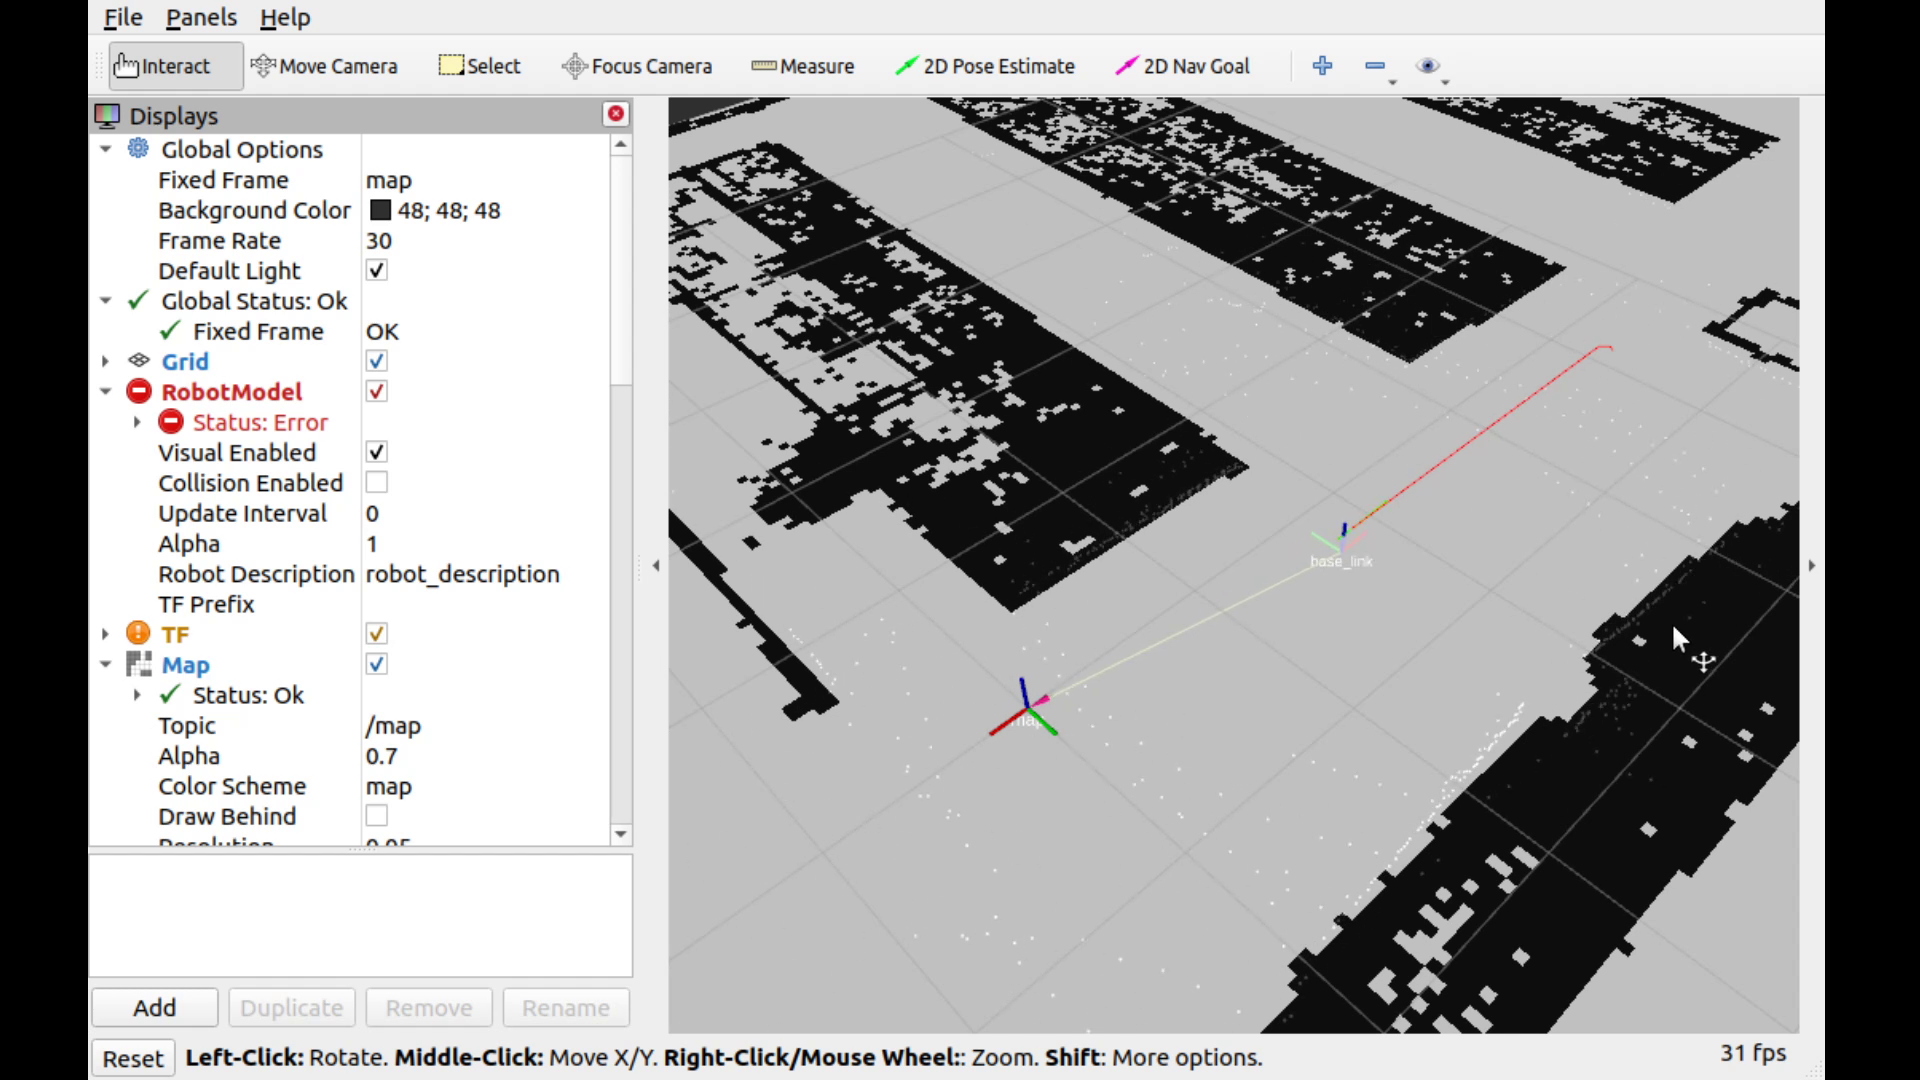
\includegraphics[width=\linewidth]{report_assets/navigation.png}
\end{minipage}\hfill
\begin{minipage}[t]{0.48\textwidth}
\centering
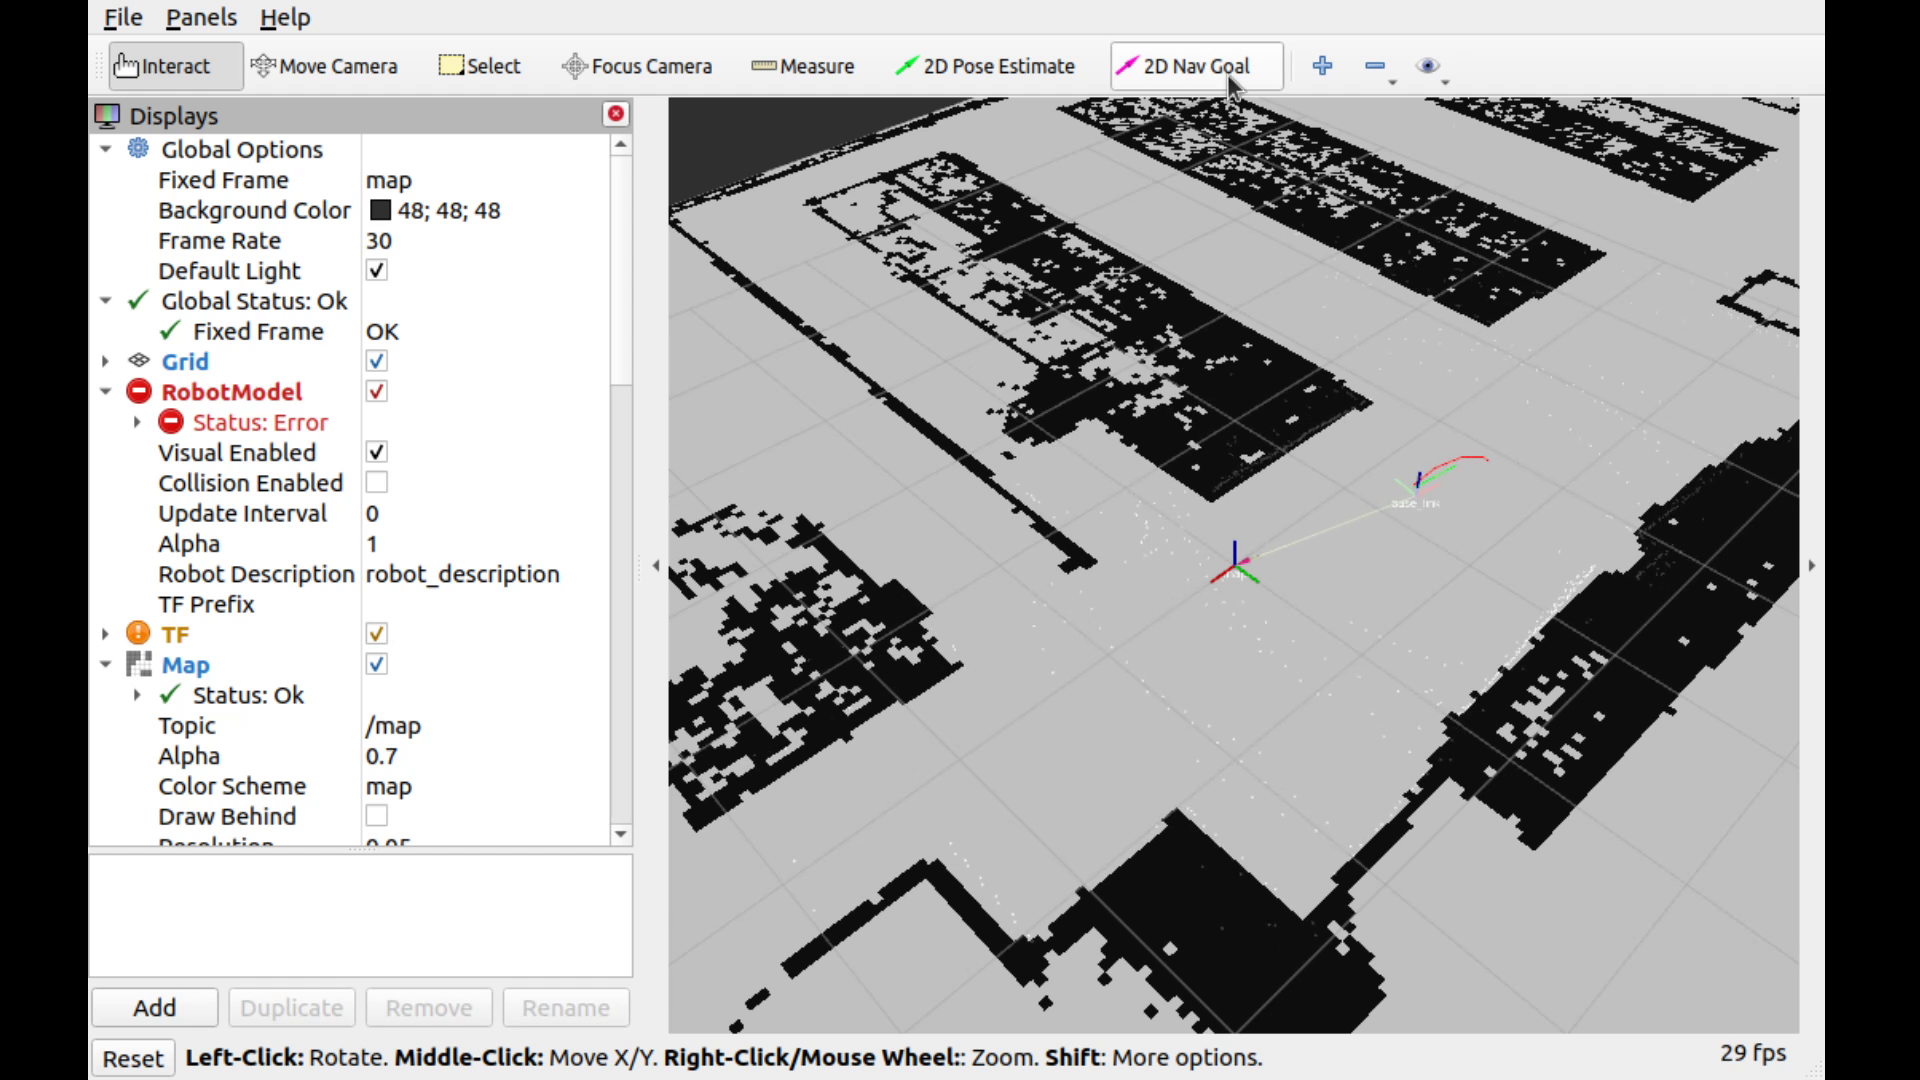
\includegraphics[width=\linewidth]{report_assets/obstacle.png}
\end{minipage}
\caption{Qualitative evidence archived during integration: a generated occupancy map used for navigation and an obstacle-avoidance visualisation captured during real experiments. These images complement the numerical benchmark by showing the practical interface between SLAM output, map use, and local obstacle handling.}
\label{fig:qualitative-nav}
\end{figure}

\begin{figure}[H]
\centering
\begin{minipage}[t]{0.48\textwidth}
\centering
\IfFileExists{/home/niumu/FYP/TF-tree/tf_liosam_baseline.pdf}{%
\includegraphics[width=\linewidth,height=0.22\textheight,keepaspectratio]{/home/niumu/FYP/TF-tree/tf_liosam_baseline.pdf}%
}{%
\fbox{\parbox[c][0.22\textheight][c]{0.9\linewidth}{\centering TF tree file unavailable during compilation}}%
}
\par\small LIO-SAM
\end{minipage}\hfill
\begin{minipage}[t]{0.48\textwidth}
\centering
\IfFileExists{/home/niumu/FYP/TF-tree/tf_fastlio_baseline.pdf}{%
\includegraphics[width=\linewidth,height=0.22\textheight,keepaspectratio]{/home/niumu/FYP/TF-tree/tf_fastlio_baseline.pdf}%
}{%
\fbox{\parbox[c][0.22\textheight][c]{0.9\linewidth}{\centering TF tree file unavailable during compilation}}%
}
\par\small FAST-LIO
\end{minipage}\vspace{0.8em}

\begin{minipage}[t]{0.48\textwidth}
\centering
\IfFileExists{/home/niumu/FYP/TF-tree/tf_pointlio_baseline.pdf}{%
\includegraphics[width=\linewidth,height=0.22\textheight,keepaspectratio]{/home/niumu/FYP/TF-tree/tf_pointlio_baseline.pdf}%
}{%
\fbox{\parbox[c][0.22\textheight][c]{0.9\linewidth}{\centering TF tree file unavailable during compilation}}%
}
\par\small Point-LIO
\end{minipage}\hfill
\begin{minipage}[t]{0.48\textwidth}
\centering
\IfFileExists{/home/niumu/FYP/TF-tree/tf_fasterlio_baseline.pdf}{%
\includegraphics[width=\linewidth,height=0.22\textheight,keepaspectratio]{/home/niumu/FYP/TF-tree/tf_fasterlio_baseline.pdf}%
}{%
\fbox{\parbox[c][0.22\textheight][c]{0.9\linewidth}{\centering TF tree file unavailable during compilation}}%
}
\par\small FASTER-LIO
\end{minipage}
\caption{Baseline TF trees archived for the four evaluated algorithms. Reviewing these trees was essential during integration because local costmap update problems often traced back not to the planner itself, but to differences in frame exposure, odometry topics, or cloud topics that had to be harmonised before fair comparison.}
\label{fig:tf-baselines}
\end{figure}

\chapter{Major Engineering Problems and Resolutions}

\section{Abrupt Teleoperation and Poor Recording Quality}
\textbf{Problem.} Early manual driving produced large velocity jumps and unstable motion, which degraded dataset quality and made repeatable evaluation difficult.

\textbf{Cause.} Raw teleoperation commands were sent directly to the base without acceleration limiting.

\textbf{Resolution.} A command smoother was implemented to enforce linear and angular acceleration/deceleration limits before publishing \texttt{/cmd\_vel}. Conservative defaults were added to the standard recording launch.

\textbf{Outcome.} Robot motion during dataset acquisition became smoother and easier to reproduce.

\section{Missing Ground Truth for ATE/RPE}
\textbf{Problem.} Early offline evaluation produced \texttt{NA} for ATE and RPE.

\textbf{Cause.} The original recording pipeline did not preserve a usable reference odometry topic.

\textbf{Resolution.} The standard recording launch was revised to include \texttt{/odom} alongside LiDAR, IMU, TF, and TF-static topics.

\textbf{Outcome.} Later static evaluation runs successfully produced valid ATE and RPE values for all four algorithms.

\section{Residual ROS Processes Breaking Repeated Runs}
\textbf{Problem.} Re-running SLAM and navigation often left behind relay or launch processes that kept printing warnings, respawning nodes, or interfering with later runs.

\textbf{Cause.} ROS child processes and relay nodes were not being shut down consistently.

\textbf{Resolution.} The unified startup script was expanded to clean process groups, kill matching relays and navigation processes, and run ROS node cleanup.

\textbf{Outcome.} Repeated experiments became much more stable and debugging became significantly easier.

\section{LIO-SAM Map Export Crash on Empty Clouds}
\textbf{Problem.} LIO-SAM could crash during map saving with an exception indicating that the input point cloud had no data.

\textbf{Cause.} The map-saving path did not guard against empty keyframe sets or empty global maps.

\textbf{Resolution.} A source-level guard was added in the map-saving path to skip saving when the relevant point sets were empty.

\textbf{Outcome.} Map export no longer crashed on empty-map cases.

\section{Local Costmap Not Updating Even When the Scan Was Visible}
\textbf{Problem.} During navigation, \texttt{/scan} could be visible in RViz while the local costmap still failed to update.

\textbf{Cause.} This turned out to be a chain-level problem rather than a single configuration error. The main causes identified were wrong cloud topics, world-frame clouds being reused for near-field obstacle generation, missing body-frame cloud publication, and frame mismatches between SLAM output and costmap expectations.

\textbf{Resolution.} The navigation bridge was standardised so that each algorithm exposed an appropriate odometry topic and an appropriate cloud for obstacle generation. Point-LIO and FASTER-LIO were particularly improved by switching navigation input to \texttt{/cloud\_registered\_body}.

\textbf{Outcome.} Local costmap behaviour became much more reliable, especially for Point-LIO and FASTER-LIO.

\section{Point-LIO and FASTER-LIO Scan Generation Failures}
\textbf{Problem.} Point-LIO and FASTER-LIO sometimes produced empty or severely delayed \texttt{/scan} output for navigation.

\textbf{Cause.} The initial setup treated them as if they could be bridged identically to FAST-LIO, but their useful cloud outputs for navigation were not identical in practice. Point-LIO initially lacked a usable body-frame cloud in the tested configuration, and FASTER-LIO exhibited delay when a world-frame registered cloud was used to regenerate a local scan.

\textbf{Resolution.} Body-frame cloud publication was enabled where necessary, and the bridge was updated to use \texttt{/cloud\_registered\_body} instead of a registered map-frame cloud.

\textbf{Outcome.} Scan availability and local costmap responsiveness improved substantially.

\section{Sensor Adaptation and Data-Format Mismatch}
\textbf{Problem.} Early integration work revealed that algorithm assumptions did not always match the available sensor outputs or ROS message formats.

\textbf{Cause.} Progress materials from the earlier reproduction phase recorded several mismatches: some algorithms assumed richer IMU information than was readily available from the working setup, some expected point-cloud data in \texttt{PointCloud2} form, and some relied on ring metadata that was not directly available in the initial processing chain.

\textbf{Resolution.} The integration workflow was gradually reshaped so that the chosen algorithms consumed data in formats they could reliably process. This included format conversion, topic restructuring, and avoiding solution paths that would require a disproportionately heavy adaptation burden relative to the project timeline.

\textbf{Outcome.} The final benchmark focused on algorithms that could be integrated reproducibly on the available hardware rather than on a theoretically broader but less tractable algorithm set.

\section{Onboard Compute and Build Stability on Raspberry Pi 3}
\textbf{Problem.} The Raspberry Pi 3 based platform could become unresponsive or run out of memory during software compilation and setup.

\textbf{Cause.} The onboard platform has limited RAM, and aggressive parallel compilation settings created memory pressure beyond what the device could comfortably support.

\textbf{Resolution.} Swap expansion and conservative compilation settings were adopted during platform preparation. This reduced build instability and enabled package preparation on the low-cost onboard computer.

\textbf{Outcome.} The platform became substantially more usable for deployment and maintenance, and the report gained a realistic low-cost deployment dimension rather than assuming workstation-class compute everywhere.

\section{Electrical and Connector Safety During Hardware Bring-Up}
\textbf{Problem.} Early hardware integration exposed awkward and potentially unsafe power and connector arrangements around the LiDAR, battery, and robot electronics.

\textbf{Cause.} A low-cost experimental platform often evolves incrementally, which can lead to temporary but risky cable routing, exposed connectors, or mechanically fragile interfaces.

\textbf{Resolution.} The hardware setup was reviewed iteratively, with attention paid to connector stability, cable routing, remote operation convenience, and keeping the sensing stack mechanically usable during repeated experiments.

\textbf{Outcome.} This reduced deployment friction and helped turn the robot from a one-off demonstration setup into a platform that could support repeated mapping and navigation experiments.

\section{LIO-SAM Rosbag Replay Jitter}
\textbf{Problem.} LIO-SAM appeared to shake or jump when replaying rosbag data.

\textbf{Cause.} The replayed bag contained \texttt{/tf} and related topics that conflicted with the live TF chain published by the currently running SLAM and robot-state publisher nodes.

\textbf{Resolution.} Replay was restricted to the raw sensor topics required by LIO-SAM, while avoiding simultaneous replay of conflicting TF data.

\textbf{Outcome.} Offline playback became much more stable and interpretable.

\section{Online Evaluation Script Failures and Logging Issues}
\textbf{Problem.} The waypoint evaluation script initially failed to create log output directories and occasionally sent goals that were not properly consumed by navigation.

\textbf{Cause.} The output directory was not always created before the first log write, and goal publication assumed an already-stable subscriber connection.

\textbf{Resolution.} The evaluator was extended to create output directories automatically, record richer event logs and timelines, and verify goal-subscriber readiness before evaluation.

\textbf{Outcome.} Online navigation experiments became easier to diagnose and reproduce.

\section{Direction-Dependent Behaviour Under Identical DWA Parameters}
\textbf{Problem.} The robot could move much faster in one world direction than the opposite direction even though the planner parameters were unchanged and the robot still moved forward in both cases.

\textbf{Cause.} The effect was traced not to DWA using different parameters, but to SLAM-dependent differences in odometry smoothness, cloud density, and obstacle representation. In particular, LIO-SAM and FAST-LIO exposed different odometry and cloud characteristics to the same navigation stack.

\textbf{Resolution.} The study shifted from treating the planner as the only cause to analysing the upstream odometry and cloud pipeline as part of the navigation system.

\textbf{Outcome.} This became an important conceptual finding of the project: the same planner parameters do not imply the same navigation behaviour when the perception and odometry inputs differ.

\chapter{Discussion}

\section{Why the Same Planner Parameters Produced Different Robot Behaviour}
One of the key lessons from this project is that a fair planner comparison requires much more than identical DWA parameters. The planner responds to the state estimate and obstacle observations it receives. Therefore, if one SLAM algorithm publishes denser clouds, more conservative near-field observations, or noisier odometry, the robot may slow down earlier or take wider detours even though the planner configuration file is unchanged.

This is precisely what was observed in the project. FAST-LIO, Point-LIO, and FASTER-LIO belong to a similar tightly coupled filter-based family, but they still needed different cloud selections to produce usable local scans. LIO-SAM, meanwhile, interacted differently with the navigation stack depending on whether the odometry source and cloud source were taken from its intermediate or mapping outputs. The project therefore shows that system-level navigation performance is a function of the whole perception-to-planning chain, not only of the planner itself.

\section{Engineering Fairness Versus Algorithm Purity}
A second lesson concerns fairness. If every algorithm is forced into exactly the same cloud topic type regardless of its intended design, the comparison may become formally uniform but practically meaningless. In this project, fairness was defined instead as follows: same robot, same map, same waypoint task, same navigation stack, same evaluation metrics, but a carefully justified and documented choice of odometry and cloud topic for each algorithm. This is a more realistic definition of fairness for system integration work.

\section{What This Project Contributes Beyond a Simple Benchmark}
A key outcome of the project is that it transforms a set of independently available open-source packages into a coherent deployment workflow. This contribution may appear less mathematically novel than a new estimator or planner, but it is highly relevant in practice. Many robotics projects fail to become reusable precisely because they stop at the level of a successful demonstration and do not standardise recording, launch, reset, evaluation, and reporting. By contrast, this project organises those steps explicitly and archives both the scripts and the outputs required to rerun them.

Another contribution is methodological. The debugging history shows that many failures initially attributed to the local planner were in fact caused by upstream representation choices such as frame conventions, wrong relay topics, or unsuitable scan generation from 3D clouds. This reinforces an important systems lesson: a planner cannot be evaluated in isolation if its sensor and odometry inputs differ substantially across runs. In this sense, the project does not simply compare four SLAM methods; it exposes how SLAM output design interacts with a classical indoor navigation stack.

\section{Implications for Low-Cost Mobile Robot Deployment}
The project title emphasises low-cost deployment, and the engineering record supports this framing. The platform combines a TurtleBot3 base, a Raspberry Pi 3 on the robot side, and a Livox MID360 sensor. This is not a high-end industrial stack, and that is precisely why deployment realism matters. On an affordable platform, every mismatch in frame naming, process startup, topic routing, and resource usage is magnified. A workflow that only works when manually nursed by the developer is not a useful deployment method.

From this perspective, the most valuable outcome is not only that certain algorithms achieved low error on a bag, but that the project now contains a reproducible path from recording to mapping to navigation to evaluation. This positions the work as both an algorithm comparison and a deployment study, which is well aligned with the original project brief.

\section{Limits of the Current Archive}
The local project archive already supports a strong report with complete static comparisons and a complete repeated online comparison for the indoor laboratory static-obstacle scenario. However, two limitations remain. First, the online quantitative archive is not yet equally complete for the outdoor and corridor scenarios across all four algorithms. Second, some qualitative evidence still exists primarily as video, debugging screenshots, or engineering notes rather than as a fully tabulated benchmark for every scenario. These limitations do not invalidate the work, but they should be stated clearly in the final report and closed by adding the remaining scenario-specific summary files and supporting figures.

\chapter{Conclusion and Future Work}
This project developed a unified benchmark platform for comparing four LiDAR-inertial SLAM algorithms on a Livox MID360 mobile robot under a shared ROS navigation stack. The work went beyond simply launching open-source packages: it established a full engineering workflow for recording, deployment, unified startup, static rosbag evaluation, online waypoint evaluation, map generation, and problem diagnosis.

The completed experiments show that the four algorithms differ not only in localisation accuracy and computational load, but also in how well their outputs support real-time local obstacle perception and navigation. In the repeated laboratory static-obstacle benchmark, Point-LIO achieved the best overall efficiency, FAST-LIO provided the strongest balance between speed, safety, and computational demand, LIO-SAM delivered the most conservative obstacle clearance together with the best positional consistency, and FASTER-LIO remained the most aggressive and least safe under the current integration. The project also demonstrated that many apparent navigation problems are in fact integration problems involving coordinate frames, cloud representations, and observation pipelines rather than failures of the planner alone.

Future work should focus on three directions. First, the same complete four-algorithm online benchmark should be executed for the outdoor and corridor scenarios so that the conclusions become fully scenario-general rather than laboratory-centric. Second, the navigation configuration should be further refined using more realistic robot footprint calibration and scenario-specific obstacle design, especially for narrow-passage corridor experiments. Third, the benchmark can be extended with repeated trials, statistical confidence intervals, and richer scenario-wise discussion so that the comparison becomes publication-ready.

\section{Immediate Next Steps for Completing the Final Comparison}
The remaining work required to turn the current draft into a fully complete final report is well defined. First, the same evaluation harness should be executed on the outdoor map and corridor map for all four algorithms so that the scenario-wise discussion can be supported by standardised summaries rather than only qualitative expectation. Second, more hardware photographs and environment photographs should be inserted so that the report visually documents the physical platform and each test setting. Third, the existing indoor laboratory benchmark can be further strengthened by adding statistical confidence intervals and perhaps one or two additional repeated trials if time allows.

This is a manageable completion path because the report structure, metric definitions, and archive conventions are already in place. In other words, the remaining work is no longer about inventing the methodology; it is mainly about filling the remaining cells of an already standardised benchmark matrix.

\appendix

\chapter{Archived Project Assets Reviewed for This Report}
The following artefacts were reviewed while drafting this report:
\begin{enumerate}[leftmargin=2em]
    \item rosbags under the local \texttt{FYP/PointCloudBag} archive,
    \item exported PCD map folders such as \texttt{maps}, \texttt{maps\_324}, and \texttt{new\_maps},
    \item TF tree snapshots under \texttt{FYP/TF-tree},
    \item online waypoint evaluation outputs under \texttt{FYP/nav\_eval\_results},
    \item static rosbag evaluation outputs under \texttt{FYP/static\_eval\_results},
    \item waypoint definitions under \texttt{FYP/waypoints},
    \item obstacle-avoidance videos under \texttt{FYP/video}, and
    \item weekly presentation materials such as \emph{Report on Last Week's Work} used to recover early design decisions, literature review scope, and hardware-integration issues.
\end{enumerate}

\chapter{Project Scripts and Their Roles}
To keep the main report concise, code is not reproduced here. Instead, the principal scripts are summarised in Table~\ref{tab:scripts}.

\begin{table}[H]
\centering
\caption{Project scripts and their roles.}
\label{tab:scripts}
\begin{tabular}{p{0.30\textwidth}p{0.58\textwidth}}
\toprule
Script or file & Main role \\
\midrule
\path{record_dataset.launch} & Standardised rosbag recording with odometry bridging and command smoothing \\
\path{cmd_vel_smoother.py} & Limits acceleration and deceleration of teleoperation commands \\
\path{run_slam_nav.sh} & Unified SLAM plus navigation startup and cleanup \\
\path{eval_static_rosbag.sh} & Batch static rosbag evaluation driver \\
\path{slam_eval_monitor.py} & Resource and frame-time monitoring during static evaluation \\
\path{bag_to_tum.py} & Converts ROS messages into TUM trajectory format \\
\path{summarize_static_eval.py} & Produces static comparison summary tables \\
\path{capture_waypoints.py} & Records waypoint routes in the map frame \\
\path{nav_waypoint_eval.py} & Single-algorithm online waypoint evaluation \\
\path{eval_nav_4alg.sh} & Batch online evaluation across four algorithms \\
\path{summarize_nav_eval.py} & Merges navigation results into summary tables \\
\path{pcd_to_grid.py} & Converts PCD map files into 2D occupancy maps \\
\bottomrule
\end{tabular}
\end{table}

\chapter{Suggested Final Editing Before Submission}
Before converting this draft into the final submitted report, the following polishing steps are recommended:
\begin{enumerate}[leftmargin=2em]
    \item replace the title-page placeholders with the official NUS information required by the department,
    \item add more selected figures from RViz, TF trees, and map outputs for the outdoor and corridor scenarios,
    \item add screenshots or still frames from obstacle-avoidance videos,
    \item archive the full outdoor and corridor online benchmark results for all four algorithms, and
    \item convert local directory references into figure numbers, table numbers, or appendix notes as needed.
\end{enumerate}

\bibliographystyle{plainnat}
\bibliography{nus_fyp_report_english_20260405}

\end{document}
